\chapter{Quantum prime factorization}
\labelChapter{quantum_prime_factorization}

\section{Preface}
\labelSection{C3_preface}

This chapter is based on the work reported in Ref.~\cite{Skosana_2021}, originally appearing in Nature Scientific Reports. It was co-authored by Professor Mark Tame and the author of this thesis. Both Professor Mark Tame and the author of this thesis conceived the idea and designed the experiments, with the author of this thesis performing the experiments. Both authors analyzed the results, contributed to the discussions and interpretations. 


\section{Introduction}
\labelSection{C3_introduction}

\lettrine[lines=3]{S}{hor's} algorithm~\cite{Shor_1997} is a quantum algorithm that provides a way of finding the nontrivial factors of an $L$-bit odd composite integer $N=pq$ in polynomial time with high probability. There is no known classical algorithm that can solve the same problem in polynomial time~\cite{Mike&Ike, Dewolf_2019}. The crux of Shor's algorithm rests upon \gls{QPE}~\cite{Mike&Ike}, which is a quantum routine that estimates the phase $\varphi_u$ of an eigenvalue $e^{2\pi i \varphi_u}$ corresponding to an eigenvector $\ket{u}$ for some unitary matrix $\hat{U}$. \acs{QPE} efficiently solves a problem related to factoring, known as the order-finding problem, in polynomial time in the number of bits needed to specify the problem, which in this case is $L=\ceil{\log_{2}{N}}$. By solving the order-finding problem using \acs{QPE} and carrying out a few extra steps, one can factor the integer $N$. 

\bigskip
\noindent
A large corpus of work has been done with regards to the experimental realization of Shor's algorithm over the years. Similar to the experimental realization of Grover's algorithm discussed in the previous chapter, the pioneering work was performed with liquid-state nuclear magnetic resonance, factoring $15$ on a $7$-qubit computer~\cite{Vandersypen_2001}. The considerable resource demands of Shor's original algorithm were circumvented by using various approaches, including adiabatic quantum computing~\cite{Peng_2008} and in the standard network model using techniques of compilation~\cite{Vidal_2003a} that reduced the demands to within the reach of single-photon architectures~\cite{Lu_2007, Lanyon_2007, Politi_2009} and a super-conducting phase qubit system~\cite{Lucero_2012}. 

\clearpage
\noindent
In 2012, a proof-of-concept demonstration of the order-finding algorithm for the integer $21$ was carried out with photonic qubits using, in addition to the aforementioned compilation technique, an iterative scheme~\cite{Lopez_2012}, where the control register is reduced to one qubit and this qubit is reset and reused~\cite{Griffiths_1996}. However, factoring was not possible in this demonstration due to the low number of iterations. Later, the iterative scheme was demonstrated for factoring 15, 21 and 35 on an IBM quantum processor by splitting up the iterations and combining the outcomes~\cite{Amico_2019}. Recently, building on previous schemes of hybrid factorization~\cite{Pal_2019, Xu_2012}, a quantum-classical hybrid scheme has been implemented on IBM's quantum processors for the prime factorization of $35$. This hybrid scheme of factorization alleviates the resource requirements of the algorithm at the expense of performing part of the factoring classically~\cite{Saxena_2021}.

\bigskip
\noindent
The main result of this chapter builds on the order-finding routine of Ref.~\cite{Lopez_2012} and implements a version of Shor's algorithm for factoring 21 using only $5$ qubits -- the work register contains 2 qubits and the control register contains $3$ qubits, each providing 1-bit of accuracy in the resolution of the peaks in the output probability distribution used to find the order. This approach is in contrast to the iterative version~\cite{Parker_2000} used in Refs.~\cite{Lopez_2012} and~\cite{Amico_2019}, which employs a single qubit that is recycled through measurement and feed-forward, giving 1-bit of accuracy each time it is recycled. The advantage of the iterative approach lies in this very reason; through mid-circuit measurement and real-time conditional feed-forward operations, the total number of qubits required by the algorithm is significantly reduced. At the time of writing, IBM's quantum processors do not yet support real-time conditionals necessary for the implementation of the iterative approach, so we use 3 qubits for the control register, one for each effective iteration. Thus, our compact approach is completely equivalent to the iterative approach. In future, once the capability of performing real-time conditionals is added, a further reduction in resources will be possible for our implementation, potentially improving the quality of the results even more and opening up the possibility of factoring larger integers.

\bigskip
\noindent
As it stands, the controlled-NOT gate count of the standard algorithm for $N=21$~\cite{Beauregard_2003} exceeds $40$. In our preliminary tests we found that the output probability distribution is indistinguishable from a uniform probability distribution (noise) on the IBM quantum processors. Our improved version reduces the controlled-NOT gate count through the use of relative phase Toffoli gates, reducing the controlled-NOT gate count by half while leaving the overall operation of the circuit unchanged and we suspect this technique may extend beyond the case considered here. We have gone further than the work in Ref.~\cite{Lopez_2012}, where full factorization of 21 was not achieved as with only two bits of accuracy for the peaks of the output probability distribution, the final step of continued fractions would fail to extract the correct order. On the other hand, in the work in Ref.~\cite{Amico_2019}, where 21 was factored on an IBM processor, a larger number of 6 qubits was required and the iterations were split into three separate circuits, with the need to re-initialise the work register into specific quantum states for each iteration. Our approach is thus more efficient and compact, enabling algorithm outcomes with reduced noise. To support our claims, we successfully carry out continued fractions and evaluate the performance of the algorithm by (i) quantitatively comparing the measured probability distribution with the ideal distribution and noise \via the Kolmogorov distance, (ii) performing state tomography experiments on the control register, and (iii) verifying the presence of entanglement across both registers.

\clearpage
\section{Background}
\labelSection{C3_background}

\subsection{Order-finding}
\labelSection{C3_order_finding}

The order-finding problem is intimately related to that of finding prime factors\footnote{A prime number is any integer greater than $1$, which only is divisible by $1$ and itself.} of a composite integer. The two problems are tied together with a few number and group theoretic results, we will follow~\cite{Mike&Ike, Dewolf_2019} and mention these in passing here.

\bigskip
\noindent
Two positive integers $N$ and $x \leq N-1$ are relatively prime to each other if they share no common factor, that is, the largest positive integer $c$ that divides both $N$ and $x$ is $1$. The integer $c$ is called the greatest common divisor of the integers $N$ and $x$, and denoted by $\gcd(x, N) =  c$; for relatively prime integers $N$ and $x$, $\gcd(x, N) = 1$. The set of positive integers $x$ that are relatively prime to $N$, form a finite Abelian group~\footnote{Multiplication of elements in the group are also in the group (closure), multiplication under the group operation is associative and commutative, the group contains a multiplicative identity with respect to the group operation and every element in the group has a unique multiplicative inverse with respect to the group operation.} with the group operation being multiplication mod $N$, this group is denoted by $\mathbb{Z}_N^{*}$. Consider an arbitrary element $x$ of $\mathbb{Z}_N^{*}$, the sequence 

\begin{align}
	\labelEquation{subgroup}
	x^{0} \text{ mod } N = 1, x^{1} \text{ mod } N,  x^{2} \text{ mod } N, x^{3} \text{ mod } N, \ldots,
\end{align}

\noindent
this sequence of elements forms a subgroup (finite) of $\mathbb{Z}_{N}^{*}$. For the subgroup to be finite implies that the above sequence will not carry on indefinitely but repeat after several iterations, that is, there exists a positive integer $r$ for which

\begin{align}
	\labelEquation{order_finding}
	x^{r} \text{ mod }N = 1,
\end{align}

\noindent
for positive integers greater than $r$, the sequence in~\refEquationOnly{subgroup} will cycle again, restarting at integer multiples of $r$. Thus the size of the subgroup is given by the smallest integer $r$ satisfying~\refEquationOnly{order_finding}, evidently $r \leq N$. Such an integer is called the order of element $x$ in $\mathbb{Z}_{N}^{*}$. The order-finding problem may be stated as follows. Given two relatively prime positive integers $N$ and $x \in \{0, 1, \ldots, N - 1\}$ , we seek to find the smallest positive integer $r \in \{0, 1, \ldots N\}$ such that $x^{r}\text{ mod } N = 1$. 

\bigskip
\noindent
It is not immediately clear how the solution to the above problem has anything at all to do with prime factorization of composite integers. To see this, suppose we were able to find an even order $r$ for two integers $N$ and $x$,

\begin{align}
	x^{r} \text{ mod } N = 1, \nonumber \\
	x^{r} - 1 \text{ mod } N = 0, \nonumber \\
	(x^{r/2})^2 - 1 \text{ mod } N = 0, \nonumber \\
	(x^{r/2} - 1)(x^{r/2} + 1) \text{ mod } N  = 0.
\end{align}

\noindent
The case where the solution to the last expression excludes both $x^{r/2} = 1$ and $x^{r/2} = N - 1$ (collectively, $x^{r/2} \text{ mod } N \neq \pm 1$) is of particular interest, since this would mean that at least one of the factors $(x^{r/2} - 1)$ and $(x^{r/2} + 1)$, which are both greater than $0$ and less than $N$, divides $N$. Computing the greatest common divisor $\gcd(x^{r/2} \pm 1, N)$, we can possibly learn at least one non-trivial prime factor of $N$, that is a factor of $N$ is only divisible by $1$ and itself only. The reasons why $\gcd(x^{r/2} \pm 1, N)$ is not always guaranteed to be a non-trivial prime factor of $N$ are the crucial assumptions leading to the result; that the found order $r$ is even so that for the chosen $x$ relatively prime to $N$, $x^{r/2} \text{ mod } N \neq \pm 1$, these two assumptions are not always true. However, they are true half of the time, it can be shown that the probability that the order $r$ is even and a randomly chosen element $x$ in $\mathbb{Z}_N^{*}$, satisfies $x^{r/2} \text{ mod } N \neq \pm  1$ is greater than one half\footnote{The interested reader may refer for a proof of this statement in Theorem A4.13 of Ref.~\cite{Mike&Ike}}. 


\clearpage
\noindent
Thus we may find a prime factorization of a composite integer $N$ with high probability, by finding the order of the group $\mathbb{Z}_{N}^{*}$. If we can efficiently compute the order of $\mathbb{Z}_{N}^{*}$, we can find an efficient algorithm to successfully compute the factors of $N$ with high probability since the preliminary steps can be also be computed efficiently\footnote{An efficient algorithm is one that computes a solution to a problem in steps/elementary operations that scale polynomially with the intrinsic size of the problem. For prime factorization, the size of problem is the  number of bits needed to specify $N$, $L \equiv \ceil{\log_{N}}$.}. For a chosen $N$, (i) we can check easily check if it is even and return $2$. (ii) We also can always check if $N=p^{m}$ is a prime power, and find $p$ efficiently. (iii) To check if a chosen $x$ is relatively prime to $N$, we compute $\gcd{(x, N)} = 1$ if not, then $\gcd{(x, N)}$ is a factor of $N$ and the $\gcd(x, N)$ may be computed efficiently as well. (iv) Lastly, we compute the order of $x\text{ mod }N$ and check if $\gcd{(x^{r/2}\pm 1, N)}$ yields a non-trivial factor of $N$, succeeding most of the time.

\bigskip
\noindent
Classically, such an algorithm that solves the order-finding problem with steps that scale polynomially in the number of bits $L \equiv \ceil{\log{N}}$ needed to specify $N$ is yet to be found~\cite{Mike&Ike, Dewolf_2019}. Here enters Shor's algorithm which efficiently solves the order-finding problem with a number of elementary operations that scale polynomially with $\ceil{\log{N}}$.

\subsection{Shor's quantum algorithm for order-finding}
\labelSection{C3_shors_quantum_algorithm_for_order_finding}

Peter Shor's insight was the realization that the order-finding problem can reduced into another related problem, for which quantum computers were known to solve efficiently, that is, with a number of elementary operations (quantum gates) that scales polynomially. The latter problem is the finding an eigenvalue $\lambda$ corresponding to an eigenvector $\ket{u}$ of a unitary matrix $U$, that is $U\ket{u} = \lambda \ket{u}$. Since $U$ is unitary ($U^{-1} = U^{\dagger}$), its eigenvalues are complex numbers with unit modulus, since

\begin{align}
	1 = \braket{u}{u} = \expval{U^{\dagger}U}{u} = \lambda^*\lambda \expval{\mathds{1}}{u} = \abs{\lambda}^2,
\end{align}

\noindent
therefore  $\lambda$ may be parametrized by $\lambda = e^{2\pi i \varphi}$ with $\varphi \in [0, 1)$. The canonical \acs{QPE} is due to Kitaev~\cite{Kitaev_1995} (and later by Cleve~\etal~\cite{Cleve_1998} in its current form) and provides an efficient way to estimate the value of $\varphi$.  The quantum algorithm for order-finding is an instance of the \acs{QPE} for the following unitary $U_x$. For two relatively prime positive integers $x$ and $N$, and for $y \in \{0, 1, 2,\ldots, N - 1\}$, the action of $U_x$ on a computational basis element $\ket{y}$ is defined by:

\begin{align}
	U_x\ket{y} = \ket{x y \text{ mod } N}.
\end{align}

\noindent
The matrix $U_x$ is unitary since $\ip{y}{y'} = \delta_{y, y'}$ and 

\begin{align}
	\matrixel{y}{U_x^{\dagger}U_x}{y'} &= \ip{xy \text{ mod } N}{xy' \text{ mod } N}, \nonumber \\
								   &= \ip{xy}{xy'}, \nonumber \\
								   &= \delta_{xy, xy'}, \nonumber \\
								   &= \delta_{y, y'}.
\end{align}

\noindent
This because if $xy = xy' \implies x^{-1}xy  = x^{-1}xy' \implies y = y'$, similarly $xy \neq xy' \implies y \neq y'$.

\clearpage
\noindent
Since $x$ is relatively prime to $N$, the multiplicative inverse $\text{ mod } N$ of $x$ exists. Recall from ~\refEquationOnly{order_finding} that if $r$ is the order of $x \text{ mod } N$, then $x^{r}\text{ mod } N = 1$, for our unitary matrix $U_x$ this means that for any computational basis state $\ket{y}$

\begin{align}
	(U_x)^r\ket{y} = \ket{x^ry \text{ mod } N} = \ket{y} \implies (U_x)^{r} = \mathds{1}
\end{align}

\noindent
From the above fact, if $\ket{u_k}$ is an eigenstate of $U_x$, then the corresponding eigenvalues are $r$-th roots of unity,

\begin{align}
	\expval{I}{u_k} = \expval{(U_x)^{r}}{u_k} = \lambda_k^r =  1, \nonumber \\
	\lambda_k = e^{2\pi i k / r},\quad k \in \{0, 1, 2, \ldots, r - 1\}.
\end{align}

\noindent
With a little of bit algebraic deadlifting one can show that the corresponding mutually orthonormal eigenvectors are given by~\cite{Mike&Ike}:


\begin{align}
	\labelEquation{eigenstate}
	\ket{u_k} = \frac{1}{\sqrt{r}} \displaystyle\sum_{q=0}^{r-1} e^{2\pi i q k / r} \ket{x^{k} y \text{ mod }N},
\end{align}

\noindent
for any $y$ in $\{0, 1, 2, \ldots, N-1\}$ (for convenience, typically $y=1$). Thus, in this instance for a given eigenstate $\ket{u_k}$ of $U_x$, the \acs{QPE} algorithm provides an estimate of $k/r$, which if we are clever enough we may extract the order $r$.

\bigskip
\noindent
Next, we summarize the \acs{QPE} algorithm; given the unitary matrix $U$ and an efficient way to apply the controlled-$U^{2^j}$ operations in terms of other elementary gates, estimate $\varphi$ for the eigenstate $\ket{u_s}$ of $U$ with eigenvalue $e^{2\pi i \varphi}$. In the case of order-finding, each of the unitaries $U^{2^j}$ carry out \emph{modular exponentiation} on a basis state:

\begin{align}
	U_x^{2^{j}}\ket{y} = \ket{x^{2^j} y \text{ mod } N}.
\end{align}

\noindent
The \acs{QPE} algorithm initially proceeds by preparing a set of $n$ qubits in the state $\ket{0}$ and a Hadamard $H$ gate is applied on each of the $n$ qubits; preparing an equal superposition state of all the possible $2^n$ computational basis states

\begin{align}
	H^{\otimes n} \ket{0}^{\otimes n} = \ket{+}^{\otimes n} = \frac{1}{\sqrt{2^n}}\displaystyle\sum_{j=0}^{2^n - 1} \ket{j}.
\end{align}

\noindent
An eigenstate $\ket{u_s}$ of the unitary matrix $U$ is prepared by another set of $m$ qubits, resulting in the joint state at beginning of the algorithm.

\begin{align}
	\labelEquation{superpos}
	\frac{1}{\sqrt{2^n}}\displaystyle\sum_{j=0}^{2^n - 1} \ket{j}\otimes\ket{u_s}.
\end{align}

\noindent
This is then followed by repeated applications of the controlled-$U$ operations, raised to successive powers of two as shown in~\refFigureOnly{qpe}. 

\clearpage

\begin{figure}[h]
	\centering
	\begin{tikzpicture}
		\begin{yquant}[register/separation=6mm]
			qubit {$b_0$} j0;
			[name=wave, register/minimum height=6mm]
			nobit wave;
			qubit {$b_1$} j1;
			qubit {$b_{2^n -1}$} j2;
			qubit {} s[3];
			init {$\ket{u_s}$} (s[-2]);
			h j0;
			vdots wave;
			h j1;
			h j2;
			box {$U^{2^{0}}$} (s) | j2;
			box {$U^{2^{1}}$} (s) | j1;
			[draw=none]
			box {$\dots$} j0,j1,j2,s;
			box {$U^{2^{n-1}}$} (s) | j0;

			output {$\ket{u_s}$} (s[0-2]);
			output {$(\ket{0} + e^{2\pi i 2^{n-1}\varphi}\ket{1})/\sqrt{2} $} j0;
			output {$(\ket{0} + e^{2\pi i 2^{1}\varphi}\ket{1})/\sqrt{2}$} j1;
			output {$(\ket{0} + e^{2\pi i 2^0\varphi}\ket{1})/\sqrt{2}$} j2;
			vdots wave;
		\end{yquant}
	\end{tikzpicture}
	\caption[Part of the \acs{QPE} routine.]{Part of the \acs{QPE} routine.}
	\labelFigure{qpe}
\end{figure}

\noindent
To see the action of this step, we consider a particular computational basis state $\ket{j}$ in the above superposition, which we can write as a bitstring $\ket{j} = \ket{b_0b_1b_2\cdots b_{n-1}}$, \ie $j = b_{0}2^{n-1} + b_1 2^{n-2} + \cdots + b_{n-2}2^{1} + b_{n-1}2^0$ (in little endian). The application of a $U^{2^i}$ is conditioned on the $i$-th ($i$-th qubit from the right most qubit) qubit being in the state $\ket{1}$, or equivalently the corresponding bit $b_{n-i}$ being $1$, otherwise it acts trivially. Thus, the action of the above step on a state $\ket{j}\otimes\ket{u_s} = \ket{b_0b_1b_2\cdots b_{n-1}}\otimes\ket{u_s}$ is

\begin{align}
	\ket{j} \otimes \ket{u_s} &\mapsto \ket{j} \otimes U^{b_{0}2^{n-1} + b_1 2^{n-2} + \cdots + b_{n-2}2^{1} + b_{n-1}2^0}\ket{u_s}, \nonumber \\
							  &= \ket{j} \otimes U^j \ket{u_s}, \nonumber \\
							  &= \ket{j} \otimes e^{2\pi i s j / r}\ket{u_s}.
\end{align} 

\noindent
By the linearity of the controlled unitaries, ~\refEquationOnly{superpos} becomes,

\begin{align}
	\labelEquation{before_iqft}
	\frac{1}{\sqrt{2^n}}\displaystyle\sum_{j=0}^{2^n - 1}e^{2\pi i s j / r}\ket{j}\otimes\ket{u_s}.
\end{align}

\noindent
In general, modular exponentiation implemented by the controlled-$U^{2^j}$ for order-finding may be realized with a number of elementary operations that scale polynomially in $L$, $\bigO{L^3}$~\cite{Mike&Ike, Cleve_1998}. The next crucial step in the \acs{QPE} algorithm is the \acs{QFT}, which is defined by its action on a computational basis state~\cite{Mike&Ike, Dewolf_2019},

\begin{align}
	\ket{j} \mapsto \frac{1}{\sqrt{2^n}} \displaystyle\sum_{k=0}^{2^n-1}e^{2\pi i j k / 2^n}\ket{k}
\end{align}

\noindent
The inverse \acs{QFT} inverts the above operation. Applying the inverse \acs{QFT} on the first set of $n$-qubits on the state in~\refEquationOnly{before_iqft}, we arrive at the following state,

\begin{align}
	\frac{1}{\sqrt{2^n}}\displaystyle\sum_{j=0}^{2^n - 1}e^{2\pi i s j / r}\ket{j}\otimes\ket{u_s} &\mapsto \ket{2^n s/r}\otimes\ket{u_s}.
\end{align}

\noindent
The \acs{QFT} (and its inverse) can be realized with two-qubit gates that asymptotically scale like $\bigO{L^2}$ \cite{Mike&Ike, Dewolf_2019}.

\clearpage
\noindent
If $s/r$ can be written exactly with $n$ bits and we proceed to measure the state above in the appropriate measurement basis, we recover the bitstring of $s/r$ with a probability of $1$, and we can subsequently extract the value of $r$ \via a continued fractions expansion. Whenever this isn't the case (\ie when $s/r$ is not a fraction of a power of two), the algorithm still yields an $n$-bit approximation of $s/r$ with high probability\footnote{The interested reader may refer to Ref.~\cite{Mike&Ike} and Ref.~\cite{Cleve_1998} for a thorough treatment of this case.}. 

\bigskip
\noindent
An assumption of the algorithm described above is that we can prepare one of the eigenstates of $U$ in~\refEquationOnly{eigenstate}, however this would require knowledge of $r$. Despite this, the algorithm still guarantees a high probability for obtaining an approximation of $s/r$. Recall that the eigenstates of $U$ form an orthonormal basis, thus any general state $\ket{\psi}$ may be expressed as

\begin{align}
	\ket{\psi} = \displaystyle\sum_{q=0}^{r-1} \alpha_q \ket{u_q}.
\end{align}

\noindent
Thus for a general $\ket{\psi}$, the probability to recover an approximation of $s/r$ for a particular $\ket{u_s}$ is simply scaled with the probability to measure that particular $\ket{u_s}$, which is $|\alpha_s|^2$. For the case of order-finding it turns out that 

\begin{align}
	\ket{1} = \frac{1}{\sqrt{r}} \displaystyle\sum_{q=0}^{r-1}\ket{u_q},
\end{align}

\noindent
and $\ket{1}$ is easy to prepare! Thus we use $\ket{1}$ in place of the $\ket{u_s}$, and when we perform a measurement at the end of the algorithm, the values of $s$ are now randomly sampled from a uniform distribution of values in $\{0, 1, 2, \ldots r-1\}$. \emph{Caveat emptor}, in such a scenario it might happen a particular $s$ shares a common factor with $r$ such that $s/r = p/q$, in which case continued fractions would incorrectly yield $q$, which we always check in constant time ($a^q \text{ mod }N = 1$). Fortunately, with enough trials, we can successfully extract $r$ in a constant number of steps. This is because for two independent trials of the algorithm yield that $s_1/r_1$ and $s_2/r_1$, respectively; if $\gcd(s_1, s_2)=1$ then the candidate value of $r$ is the least common multiple of $r_1$ and $r_2$, and the probability that $\gcd(s_1, s_2) = 1$ for two independent trials is greater than $0.25$~\cite{Mike&Ike}.


\bigskip
\noindent
The total cost of the order-finding quantum algorithm scales polynomially with $L$, with most of the cost being due to the modular exponentiation operation which requires $\bigO{L^3}$ quantum gates~\cite{Mike&Ike}. The continued fractions is classically realized with atomic steps that scale similarly. We conclude this section by summarizing Shor's quantum algorithm for order-finding:

\bigskip
\noindent
Shor's algorithm for order-finding uses two quantum registers; a control register and a work register. The control register contains $n$ qubits, each for one bit of precision in the algorithmic output. The work register contains $m = \ceil{\log{N}}$ qubits where $m$ is the number of qubits to encode $N$. The measurement of the control register outputs a probability distribution peaked at approximately the values of $2^n s/r$, where $s$ is associated with the outcome of the measurement and thus randomly assigned. The details of how the peaked probability distribution comes about are given in the order-finding routine outlined below. One can determine the order $r$ from the peak values of the distribution using continued fractions, with a number of steps that scales polynomially in $\ceil{\log{N}}$, $\bigO{L^3}$. 


\clearpage
\noindent
The procedure, or routine, for order finding is summarized below.

\begin{figure}[t]
	\centering
	\begin{tikzpicture}
		\begin{yquant}[register/separation=8mm]
			qubit {$\ket{0}^{\otimes n}$} q0;
			qubit {$\ket{1}^{\otimes m}$} q1;
			hspace {0.10cm} -;
			slash q0;
			slash q1;

			hspace {0.5cm} -;
			box {$H^{\otimes n}$} q0;

			[y radius=0.5cm]
			[x radius=0.5cm]
			box {$U_x^{2^j}$} q1 | q0;

			[y radius=0.25cm]
			[x radius=0.25cm]
			box {$QFT^{\dagger}$} q0;

			hspace {0.25cm} -;
			measure q0;
		\end{yquant}
	\end{tikzpicture}
    \caption[Circuit diagram schematic of the routine used for the period finding part of Shor's algorithm.]{Circuit diagram schematic of the routine used for the period finding part of Shor's algorithm. The first (control) register has $n$ qubits. The number of qubits in the control register determines the bit-accuracy of the value of $2^ns/r$. The bottom (work) register has the $m$ qubits required to encode $N$. First, the control and work registers are initialized, then conditional modular exponentiation is performed, indicated by the controlled unitary and an inverse quantum Fourier transform is applied to the control register followed by a standard computational basis measurement. The circuit is essentially the \acs{QPE} algorithm applied to the unitary matrix $\hat{U}_x$ -- see text for details.}
    \labelFigure{schematic}
\end{figure}

\begin{enumerate}
\item \emph{Initialization}\newline
Prepare $\ket{0}^{\otimes n}\ket{0}^{\otimes m}$ and apply $H^{\otimes n}$ on the control register and $X^{\otimes m}$ on the $m^\text{th}$ qubit in the work register to create a superposition of $2^n$ states in the control register and $\ket{1}^{\otimes m}$ in the work register:
\begin{align*}
    \ket{0}^{\otimes n}\ket{0}^{\otimes m}\to \frac{1}{2^{n/2}}\displaystyle\sum_{j=0}^{2^n-1} \ket{j}\ket{1}^{\otimes m}.
\end{align*}

\item \emph{Modular exponentiation}\newline
Conditionally apply the unitary operation $\hat{U}$ that implements the modular exponentiation function $x^j\>\text{mod}\>N$ on the work register whenever the control register is in state $\ket{j}$:
\begin{align*}
    \frac{1}{2^{n/2}} \displaystyle\sum_{j=0}^{2^n -1} \ket{j}\ket{1} & \to \frac{1}{2^{n/2}}\displaystyle\sum_{j=0}^{2^n-1}
    \ket{j}\ket{x^j\>\text{mod}\>N} \\
    & =
    \frac{1}{\sqrt{r2^n}}\displaystyle\sum_{s=0}^{r-1}\displaystyle\sum_{j=0}^{2^n-1}
    e^{2\pi i s j / r}\ket{j}\ket{u_s}. \\
\end{align*}
In the second line, $\ket{u_s}$ is the eigenstate of $\hat{U}: \hat{U}\ket{u_s} = e^{2\pi i s/r}\ket{u_s}$ and $\frac{1}{\sqrt{r}}\displaystyle\sum_{s=0}^{r-1}\ket{u_s} = \ket{1}$ has been used for the work register. This provides an alternative way to write the output state and allows a connection between the modular exponentiation operation and the \acs{QPE} algorithm for the unitary operation $\hat{U}$. \label{itm:second}

\item \emph{Inverse Quantum Fourier Transform} (\acs{QFT})\newline
Apply the inverse quantum Fourier transform on the control register:
\begin{align*}
    \frac{1}{\sqrt{r2^n}}\displaystyle\sum_{s=0}^{r-1}\displaystyle\sum_{j=0}^{2^n-1}
    e^{2\pi i s j / r}\ket{j}\ket{u_s} \to \frac{1}{\sqrt{r}}\displaystyle\sum_{s=0}^{r - 1}\ket{\varphi_s}\ket{u_s}.
\end{align*}

\item \emph{Measurements}\newline
    Measure the control register in the computational basis, yielding peaks in the probability for states where $\varphi_s \simeq 2^n s / r$ due to the inverse \acs{QFT}. Thus, the outcome of the algorithm is probabilistic, however, there is a high probability of obtaining the location of the $\varphi_s$ peaks after only a few runs. The accuracy of $\varphi_s$ to $2^{n} s / r$ is determined by the number of qubits in the control register.

\item \emph{Continued fractions}\newline
    Apply continued fractions to $\varphi=\varphi_s/2^n$ (the approximation of $s / r$) to extract out $r$ from the convergents (see~\refSectionOnly{continued_fractions} of technical~\refAppendixOnly{appendix_B} for details).

\end{enumerate}


\section{Compiled Shor's quantum algorithm for order-finding}
\labelSection{C3_compiled_shors_quantum_algorithm_for_order_finding}
As mentioned in the previous section the most resource intensive part of Shor's quantum algorithm for order-finding is modular exponentiation, which is implemented by the controlled unitaries, thus an analysis of the resource demands for the algorithm are mostly to analyze the resource demands of the modular exponentiation function. We have seen that the controlled unitaries can be implemented with $\bigO{L^3}$ elementary quantum gates. However, the preceding analysis may take for granted the physical implementations of elementary gates. In Ref.~\cite{Vedral_1996}, a full-scale implementation of Shor's algorithm to factor an $L$-bit number would require a quantum circuit with $\bigO{L^3}$ elementary quantum gates acting on $7L + 1$ qubits for the modular exponentiation. Here, the elementary gates are taken to be a single-qubit Pauli-$X$ operation, a two-qubit controlled-X operation, and a Toffoli gate. Beckman~\etal~\cite{Beckman_1996} devised a circuit for modular exponentiation that uses $5L + 1$ qubits and $72L^3$ similarly defined elementary gates, \ie factoring $N=21$ would require $9000$ elementary quantum gates acting on $26$ qubits. An improvement of both of these schemes is due to Zalka~\cite{Zalka_1998}, which uses $3L$ qubits and $\bigO{L^3}$ Toffoli gates. the modular exponentiation circuit due to Beauregard~\cite{Beauregard_2003} uses $2L + 3$ qubits and $\bigO{L^3\log(L)}$ elementary gates with a circuit depth of $\bigO{L^3}$, which represents a slight improvement over the previous schemes\footnote{The circuit depth is the number of consecutive parallel operations from input to output (measurement). Each such parallel operation can be counted as a single step, and thus depth is a proxy for algorithmic time.}.


\bigskip
\noindent
The overriding assumptions in the analysis of these schemes are (i) the underlying physical implementation of a QC has a high connectivity between its qubits and (ii) that the physical implementations natively implement a Toffoli gate, and thus may be taken to be an elementary gate. However, for modern-day \acs{NISQ} physical implementations, these two assumptions do not necessarily hold. For instance, superconducting-qubit based architectures implement a set of single-qubit gates along with a high-fidelity single two-qubit entangling gate~\cite{Kjaergaard_2020}, for which a $n$-qubit Toffoli gate is then decomposed into single and two-qubits from such a native set~\cite{Barenco_1995}. The canonical decomposition of a three-qubit Toffoli gate uses six controlled-NOT (recall~\refFigureOnly{control_control_z} in the previous chapter) and for a general $n$-qubit Toffoli gate without the use auxiliary of qubits\footnote{Recall from the previous chapter that if auxiliary qubits are permitted, a $n$-qubit Toffoli gate can be realized with $\bigO{n}$ elementary gates.}, its exact controlled-NOT count is not known~\cite{Shende_2008,Yu_2013}. Taking this into consideration, and while even ignoring the difficulties that arise from compiling such circuits on physical devices with limited connectivity, the cost of implementing these circuits on a near-term devices is significantly increased if the cost analysis of the previous schemes is done in terms of two-qubit gates.


\bigskip
\noindent
The overhead in quantum gates comes from the modular exponentiation function part of the algorithm, while the overhead in qubits comes from the level of accuracy needed to successfully carry out the continued fractions part of the algorithm. Such an overhead obviously puts a full-scale implementation beyond the reach of current devices. However, compilation techniques such as the one described in Ref.~\cite{Beckman_1996}, bridge this gap and allow for small-scale proof-of-concept demonstrations, where the quantum circuit is tailored around properties of the number to be factored. This significantly simplifies the controlled-operations that realize the modular exponentiation operation (see ~\refSectionOnly{C3_shors_quantum_algorithm_for_order_finding}), which is the most resource-intensive part of the order-finding routine. The resource demands (mostly two-qubit gates) of the compiled quantum circuit are significantly reduced, making it suitable for NISQ quantum devices with low connectivity and moderate two-qubit gate errors.

\clearpage
\noindent
From Ref.~\cite{Lopez_2012}, we extend the compiled quantum order-finding routine for the particular case of factoring $N = 21$ with $x=4$ to accommodate another iteration for better precision in the resolution of the peaks for the value of $2^ns /r$. For the case of $N=21$, other choices of $x$ give $2$, $4$ or $6$ for $r$. The cases for $r=2$ or $r=4$ have been demonstrated for $N=15$~\cite{Vandersypen_2001, Lu_2007, Lanyon_2007, Politi_2009, Lucero_2012} and would bear a similar circuit structure in the present case. With only three iterations, $r=6$ would be out of reach as continued fractions would fail. For $x=4$ we have $r=3$, which is a choice that does not suffer from the aforementioned reasons. Despite $r$ being an odd integer, the algorithm is successful in finding it from $x=4$. This is the case for certain choices of perfect square $x$ and odd $r$, and $x=4$ and $r=3$ is such a case\footnote{See Ref.~\cite{Lawson_2015} and supplementary information of Ref.~\cite{Lopez_2012} for more details.}. 

\bigskip
\noindent
In contrast to Ref.~\cite{Lopez_2012}, our implementation is not iterative and uses three qubits for the control register rather than one qubit recycled on every iteration. The iterative version is based on the recursive phase estimation, made possible by the use of the semi-classical inverse \acs{QFT}~\cite{Griffiths_1996}, which replaces two-qubit gates in the circuit with single-qubit rotations classically conditioned on the measurement outcomes, reducing the cost of circuit to $\bigO{L\log(L)}$ single-qubit gates. However, we have used the traditional inverse \acs{QFT} because mid-circuit measurements with real-time conditionals are not possible yet on IBM's quantum processors. The traditional inverse \acs{QFT} for $3$ qubits is realized by the circuit below~\cite{Mike&Ike}

\begin{figure}[h]
	\centering
	\begin{tikzpicture}
		\begin{yquant}[register/separation=6mm]
			qubit {} a;
			qubit {} b;
			qubit {} c;

			h c;
			box {$S^{\dagger}$} c | b;
			box {$T^{\dagger}$} c | a;
			h b;
			box {$S^{\dagger}$} b | a;
			h a;
		\end{yquant}
	\end{tikzpicture}
	\caption[Circuit diagram for the three-qubit inverse \acs{QFT}]{Circuit diagram for the three-qubit inverse \acs{QFT}. Here, up to a global phase, ${S^{\dagger}= R_z(-\frac{\pi}{2})}$ and ${T^{\dagger} = R_z(-\frac{\pi}{4})}$ are phase and ${\pi/8}$ gates, respectively.}
\end{figure}

\noindent
In the case where the inverse \acs{QFT} is performed before a set of measurement, we can replace the controlled gates in the above circuit to ones that are classically controlled by a preceding measurement outcome~\cite{Griffiths_1996}, and we are able to reset qubits back to $\ket{0}$ during a computation, then the above circuit can be made to use a single qubit~\cite{Parker_2000}

\begin{figure}[h]
	\centering
	\begin{tikzpicture}
		\begin{yquant}
		qubit {$\ket{0}$} s;
		cbit {$c_{\idx} = 0$} c[3];
		h s;
		measure s;
		cnot c[0] | s;
		discard s; % to suppress wires extending until re-initialization

		init {$\ket{0}$} s;
		h s;
		box {$S^{\dagger}$} s | c[0];
		measure s;
		cnot c[1] | s;
		discard s; % to suppress wires extending until re-initialization

		init {$\ket{0}$} s;
		h s;
		box {$T^{\dagger}$} s | c[0];
		box {$S^{\dagger}$} s | c[1];
		measure s;
		cnot c[2] | s;

		\end{yquant}
	\end{tikzpicture}
	\caption[Circuit diagram for the three-qubit semi-classical inverse \acs{QFT}.]{Circuit diagram for the three-qubit semi-classical inverse \acs{QFT} that recycles a single qubit and replaces the two-qubit gates in the fully coherent \acs{QFT} with classically controlled gates by the preceding measurement outcomes. Here, up to a global phase, ${S^{\dagger}= R_z(-\frac{\pi}{2})}$ and ${T^{\dagger} = R_z(-\frac{\pi}{4})}$ are phase and ${\pi/8}$ gates, respectively.}
\end{figure}


\noindent
The latter is the semi-classical \acs{QFT} that makes possible the implementation of the iterative version of Shor. If mid-circuit measurements with real-time conditionals were possible, the $3$-qubit semi-classical \acs{QFT} would be possible and may improve the quality of the results we present here through the use of only $1$ qubit for the control register, as in Ref.~\cite{Lopez_2012}. IBM has suggested that the behaviour of real-time conditionals can be reproduced through post selection of the mid-circuit measurements. However, in the present case the speed up gained would be lost using this post selection method (see ~\refSectionOnly{postselection_scaling} of technical~\refAppendixOnly{appendix_B} for details).

\bigskip
\noindent
A step that is unique to the demonstration in Ref.~\cite{Lopez_2012}, among the compilation steps of previous demonstrations, and central to their demonstration is mapping the three levels $\ket{1}$, $\ket{4}$ and $\ket{16}$ accessed by the possible $2^L=2^5$ levels of the work-register to only a single qutrit system. 

\clearpage
\noindent
In our demonstration we also use this step, however IBM processors consist of qubits and so we represent the work register by 3 basis states from a two-qubit system and discard the fourth basis state as a null state. The states encoding the three possible levels of the work register; $\ket{1}$, $\ket{4}$ and $\ket{16}$ are mapped to $\ket{q_0q_1}$ according to

\begin{align}
    \ket{1}  & \mapsto \ket{\log_{4}1}  =\ket{00}, \nonumber \\
    \ket{4}  & \mapsto \ket{\log_{4}4}  =\ket{01}, \nonumber \\
    \ket{16} & \mapsto \ket{\log_{4}16} =\ket{10}.
\end{align}

\noindent
Therefore instead of evaluating $4^j\>\text{mod}\>21$ in the work register as described in step~\ref{itm:second} of the order-finding routine, the compiled version of Shor's algorithm effectively evaluates $\log_{4}[4^j\>\text{mod}\>21]$ in its place for $j = 0,1\dots2^3-1$~\cite{Beckman_1996}, which reduces the size of the work register to $2$ qubits in comparison to the $5$ qubits required in the standard construction. Note the ordering of quantum bits in the work register is $\ket{q} = \ket{q_0}\ket{q_1}$, where the rightmost qubit is associated with the least significant bit. Similarly, with the control register we have $\ket{c} = \ket{c_0}\ket{c_1}\ket{c_2}$. In total the algorithm requires 5 qubits: 3 for the control register and 2 for the work register. Implementing the controlled unitaries $\hat{U}^x$ that perform the modular exponentiation $\ket{j}\ket{y} \to \ket{j}\hat{U}^j_x\ket{y}=\ket{j}\ket{x^j y\>\text{mod}\>N}$ reduces to effectively swapping around the states $\ket{1}$, $\ket{4}$ and $\ket{16}$ in the work register controlled by the corresponding bit of the integer $j$ in the control register, which is given by $x=c_22^0 + c_12^1 + c_02^2$. In other words, $\hat{U}^j=\hat{U}^{c_02^2}\hat{U}^{c_12^1}\hat{U}^{c_22^0}$. Thus, depending on the control qubit $c_i$, one of the following maps is applied:

\begin{align}
    \hat{U}^{1}: \{ \ket{1} \mapsto \ket{4},  \ket{4} \mapsto \ket{16}, \ket{16} \mapsto \ket{1} \}, \nonumber \\
    \hat{U}^{2}: \{ \ket{1} \mapsto \ket{16}, \ket{4} \mapsto \ket{1},  \ket{16} \mapsto \ket{4} \}, \nonumber \\
    \hat{U}^{4}: \{ \ket{1} \mapsto \ket{4},  \ket{4} \mapsto \ket{16}, \ket{16} \mapsto \ket{1} \}.
\end{align}

\noindent
The next simplification step comes from the fact that these operations on the work register need not be controlled SWAP (Fredkin) gates, they can be as simple as controlled-NOT gates, as we show next.

%%%%%%%%%%%%%%%%%%%%%%%%%%%
%%%%%%%%%%%%%%%%%%%%%%%%%%%

\subsection{Modular exponentiation}
\labelSection{C3_modular_exponentiation}

Implementing $\hat{U}^{1}$ on the two-qubit work register is simplified considerably by noting that the states $\ket{4}$ and $\ket{16}$ initially have zero amplitude, and thus the operation $\ket{1} \mapsto \ket{4}$ alone is sufficient. This operation can realized with a controlled-NOT gate controlled by $\ket{c_2}$ targeting the second work qubit $\ket{q_1}$, as shown~\refFigureOnly{U1}

\begin{figure}[h]
	\centering
	\begin{tikzpicture}
		\begin{yquantgroup}[register/separation=6mm]
			\registers{
				qubit {} c;
				qubit {} q[2];
			}
			\circuit{
				init {$\ket{c_2}$} c;
				init {$\ket{q_0}$} q[0];
				init {$\ket{q_1}$} q[1];
				box {$U^{2^0}$} (q) | c;
			}
			\equals
			\circuit{
				cnot q[1] | c;
			}
		\end{yquantgroup}
	\end{tikzpicture}
	\caption[Decomposition of the controlled-$U^{2^0}$ unitary]{Decomposition of the controlled-$U^{2^0}$ unitary as only a single controlled-NOT gate.}
	\labelFigure{U1}
\end{figure}

\noindent
Similarly, the implementation of $\hat{U}^{2}$ can be simplified by noting that the states $\ket{1}$ and $\ket{4}$ are the only non-zero amplitude states in the work register after $\hat{U}^1$ may have been applied, thus prompting us to only consider $\ket{1} \mapsto \ket{16}$ and $\ket{4} \mapsto \ket{1}$. A controlled-NOT gate controlled by $\ket{c_1}$ targeting $\ket{q_1}$ followed by a Fredkin gate, swapping $\ket{q_0}$ and $\ket{q_1}$ realizes this simplified $\hat{U}^{2}$, as shown in~\refFigureOnly{U2}

\clearpage

\begin{figure}[h]
	\centering
	\begin{tikzpicture}
		\begin{yquantgroup}[register/separation=6mm]
			\registers{
				qubit {} c;
				qubit {} q[2];
			}
			\circuit{
				init {$\ket{c_1}$} c;
				init {$\ket{q_0}$} q[0];
				init {$\ket{q_1}$} q[1];
				box {$U^{2^1}$} (q) | c;
			}
			\equals
			\circuit{
				cnot q[1]  | c;
				cnot q[0]  | q[1];
				cnot q[1]  | c,q[0];
				cnot q[0]  | q[1];
			}
		\end{yquantgroup}
	\end{tikzpicture}
	\caption[Circuit diagram showing the decomposition of the controlled-$U^{2^1}$ unitary]{Circuit diagram showing the decomposition of the controlled-$U^{2}$ unitary in terms of a Toffoli gate and two controlled-NOT gates.}
	\labelFigure{U2}
\end{figure}

\noindent
In~\refFigureOnly{U2}, the Fredkin gate has been decomposed into a Toffoli gate and two controlled-NOT gates. The subsequent implementation of $\hat{U}^{4}$ admits no simplifications as all the possible states in the work register may have non-zero amplitude at this point. This operation is implemented with a Toffoli gate and a Fredkin gate with single-qubit Pauli-$X$ gates, shown in~\refFigureOnly{U4}

\begin{figure}[h]
	\centering
	\begin{tikzpicture}
		\begin{yquantgroup}[register/separation=6mm]
			\registers{
				qubit {} c;
				qubit {} q[2];
			}
			\circuit{
				init {$\ket{c_0}$} c;
				init {$\ket{q_0}$} q[0];
				init {$\ket{q_1}$} q[1];
				box {$U^{2^2}$} (q) | c;
			}
			\equals
			\circuit{
				x q[1];
				cnot q[0] | c, q[1];
				x q[1];
				cnot q[1]  | c;
				cnot q[0]  | q[1];
				cnot q[1]  | c,q[0];
				cnot q[0]  | q[1];
			}
		\end{yquantgroup}
	\end{tikzpicture}
	\caption[Circuit diagram showing the decomposition of the controlled-$U^{2^2}$ unitary ]{Circuit diagram showing the decomposition of the controlled-$U^{2^2}$ unitary in terms of two Toffoli gates, three controlled-NOT gates and two single-qubit gates.}
	\labelFigure{U4}
\end{figure}

\noindent
The full circuit diagram is shown in~\refFigureOnly{compiled_circ} -- note that before simplification the order of application of the controlled unitaries is interchangeable, $\hat{U}^{2^{(n-1)}}$ or $\hat{U}^{2^{1}}$ could be applied first. Interchanging the order only has the effect of interchanging the order of the outcome bits at the end of the computation. This is the reason the order of application of the controlled unitaries here is in reverse order to that in Ref.~\cite{Lopez_2012}.

\begin{figure}[h]
	\centering
	\resizebox{1.0\textwidth}{!}{%
	\begin{tikzpicture}
		\begin{yquant}[register/separation=2mm]
			qubit {$\ket{\reg_{\idx}}$} c[3];
			qubit {$\ket{\reg_{\idx}}$} q[2];

			h c;
			[this subcircuit box style={draw, dashed, inner ysep=6pt, label=below:$U^{2^0}$}]
			subcircuit {
				qubit {} a;
				qubit {} b;
				qubit {} c;
				cnot c | a;
			} (c[2], q[0], q[1]);
			[this subcircuit box style={draw, dashed, inner ysep=6pt, label=below:$U^{2^1}$}]
			subcircuit {
				qubit {} a;
				qubit {} b;
				qubit {} c;
				qubit {} d;

				cnot d | a;
				cnot c | d;
				cnot d | a, b;
				cnot c | d;
			} (c[1], c[2], q[0], q[1]);
			[this subcircuit box style={draw, dashed, inner ysep=6pt, label=below:$U^{2^2}$}]
			subcircuit {
				qubit {} a;
				qubit {} b;
				qubit {} c;
				qubit {} d;
				qubit {} e;

				x d;
				cnot d | a, e;
				x d;
				cnot e | d;
				cnot d | a, e;
				cnot e | d;
			} (-);
			[this subcircuit box style={draw, dashed, inner ysep=6pt, label=above:$QFT^{\dagger}$}]
			subcircuit {
				qubit {} a;
				qubit {} b;
				qubit {} c;

				h c;
				box {$S^{\dagger}$} c | b;
				box {$T^{\dagger}$} c | a;
				h b;
				box {$S^{\dagger}$} b | a;
				h a;
			} (c);

			measure c;
		\end{yquant}
	\end{tikzpicture}
	}
	\caption[Compiled quantum order-finding routine for ${N = 21 \text{ and } x = 4}$.  This circuit uses five qubits in total; $3$ for the control register and $2$ for the work register.]{Compiled quantum order-finding routine for ${N = 21 \text{ and } x = 4}$.  This circuit uses five qubits in total; $3$ for the control register and $2$ for the work register. The above circuit determines ${2^ns/r}$ to three bits of accuracy, from which the order can be extracted. Here, up to a global phase, ${S= R_z(\frac{\pi}{2})}$ and ${T = R_z(\frac{\pi}{4})}$ are phase and ${\pi/8}$ gates, respectively.
	     }
    \labelFigure{compiled_circ}
\end{figure}

%%%%%%%%%%%%%%%%%%%%%%%%%%%
%%%%%%%%%%%%%%%%%%%%%%%%%%%

\subsection{Modular exponentiation with relative phase Toffolis}
\labelSection{C3_modular_exponentiation_with_relative_phase_Toffolis}

In total, the modular exponentiation routine requires three Toffoli gates; traditionally a single Toffoli gate can be decomposed into six controlled-NOT gates and several single-qubit gates, the decomposition is equivalent to the one shown in~\refFigureOnly{control_control_z} modulo two single qubit gates ($HZH = X$)

\begin{figure}[h!]
	\centering
	\begin{tikzpicture}
		\begin{yquantgroup}[register/separation=4mm]
			\registers{
				qubit {} c;
				qubit {} q[2];
			}
			\circuit{
				cnot q[1] | c, q[0];
			}
			\equals
			\circuit{
				h q[1];
				cnot q[1] | q[0];
				box {$T^\dagger$} q[1];
				cnot q[1] | c;
				box {$T$} q[1];
				cnot q[1] | q[0];
				box {$T^\dagger$} q[1];
				cnot q[1] | c;
				box {$T$} q[1];
				h q[1];
				box {$T$} q[0];
				cnot q[0] | c;
				box {$T^\dagger$} q[0];
				box {$T$} c;
				cnot q[0] | c;
			}
		\end{yquantgroup}
	\end{tikzpicture}
	\caption[Circuit diagram showing the decomposition of a Toffoli gate]{Circuit diagram showing the decomposition of a Toffoli gate in terms of elementary gates; six controlled-NOT gate and seven $T/T^{\dagger}$ gates.}
	\labelFigure{toffoli}
\end{figure}

\noindent
Taking into account a given processor's topology and the constraints it poses, as well as other parts of the circuit (the inverse \acs{QFT}), further increases the tally of controlled-NOT gates. 

\clearpage
\noindent
This becomes undesirable as it is understood that there is an upper limit on the number of controlled-NOT gates that can be in a circuit with the guarantee of a successful computation on \acs{NISQ} processors, with current limit is understood to be around $30$ controlled-NOT gates for IBM Q processors~\cite{Gwinner_2020,Zhang_2021}. The number of controlled-NOT gates from the decomposition of the Toffoli gate can be cut in half if we permit the operation to be correct up to relative phase shifts. Margolus constructed a gate that implements the Toffoli gate up to a relative phase shift of $\ket{101} \mapsto -\ket{101}$ that only uses three controlled-NOT gates and four single qubit gates~\cite{Marg_1994}. This construction has been shown to be optimal~\cite{Song_2003}. 

\begin{figure}[h]
	\centering
	\begin{tikzpicture}
		\begin{yquantgroup}[register/separation=6mm]
			\registers{
				qubit {} c;
				qubit {} q[2];
			}
			\circuit{
				box {$M$} q[1] | c, q[0];
			}
			\equals
			\circuit{
				box {$G$} q[1];
				 cnot q[1] | q[0];
				box {$G$} q[1];
				 cnot q[1] | c;
				box {$G^{\dagger}$} q[1];
				 cnot q[1] | q[0];
				box {$G^{\dagger}$} q[1];
			}
		\end{yquantgroup}
	\end{tikzpicture}
	\caption[Circuit diagram showing the decomposition of a Margolus gate]{Circuit diagram showing the decomposition of a Margolus gate in terms of elementary gates; three controlled-NOT and four ${G = R_y(\pi/4)}$ single qubit gates, where ${R_y(\pi/4) = e^{-i \pi / 8} S H T H S Z}$,\\ ${S=\mathrm{diag}(1, i)}$ and ${Z=\mathrm{diag}(1,-1)}$.}
	\labelFigure{margolus}
\end{figure}

\bigskip
\noindent
Maslov showed the advantages of using a relative phase Toffoli gate when the gate is applied last or when relative phases do not matter for certain configurations of Toffolis, resulting in no overall change to the functionality in any significant way~\cite{Maslov_2016}. The configuration in the circuit shown in~\refFigureOnly{compiled_circ} is one such configuration that permits a replacement of Toffoli gates with Margolus gates without changing the overall functionality. All the Margolus gates in the circuit in~\refFigureOnly{improved_circ} (which is the circuit in~\refFigureOnly{compiled_circ} with the Toffoli gates replaced by Margolus gates) never encounter the basis state $\ket{101}$, thus leaving the operation of the circuit unchanged. See~\refSectionOnly{effect_of_relative_toffolis} of technical~\refAppendixOnly{appendix_B} for details. This further compacting reduces the number of controlled-NOT gates considerably and puts the algorithm within reach of current IBM processors with a limited number of noisy qubits.

\begin{figure}[h!]
	\centering
	\resizebox{1.0\textwidth}{!}{%
	\begin{tikzpicture}
		\begin{yquant}[register/separation=2mm]
			qubit {$\ket{\reg_{\idx}}$} c[3];
			qubit {$\ket{\reg_{\idx}}$} q[2];

			h c;
			[this subcircuit box style={draw, dashed, inner ysep=6pt, label=below:$U^{2^0}$}]
			subcircuit {
				qubit {} a;
				qubit {} b;
				qubit {} c;
				cnot c | a;
			} (c[2], q[0], q[1]);
			[this subcircuit box style={draw, dashed, inner ysep=6pt, label=below:$U^{2^1}$}]
			subcircuit {
				qubit {} a;
				qubit {} b;
				qubit {} c;
				qubit {} d;

				cnot d | a;
				cnot c | d;
				box {$M$} d | a, b;
				cnot c | d;
			} (c[1], c[2], q[0], q[1]);
			[this subcircuit box style={draw, dashed, inner ysep=6pt, label=below:$U^{2^2}$}]
			subcircuit {
				qubit {} a;
				qubit {} b;
				qubit {} c;
				qubit {} d;
				qubit {} e;

				x d;
				box {$M$} d | a, e;
				x d;
				cnot e | d;
				box {$M$} d | a, e;
				cnot e | d;
			} (-);
			[this subcircuit box style={draw, dashed, inner ysep=6pt, label=above:$QFT^{\dagger}$}]
			subcircuit {
				qubit {} a;
				qubit {} b;
				qubit {} c;

				h c;
				box {$S^{\dagger}$} c | b;
				box {$T^{\dagger}$} c | a;
				h b;
				box {$S^{\dagger}$} b | a;
				h a;
			} (c);

			measure c;
		\end{yquant}
	\end{tikzpicture}
	}
    \caption[Approximate compiled quantum order-finding routine implemented with Margolus gates in place of Toffoli gates.]{Approximate compiled quantum order-finding routine implemented with Margolus gates in place of Toffoli gates in the construction in~\protect\refFigureOnly{compiled_circ}.}
    \labelFigure{improved_circ}
\end{figure}

%%%%%%%%%%%%%%%%%%%%%%%%%%%
%%%%%%%%%%%%%%%%%%%%%%%%%%%
%%%%%%%%%%%%%%%%%%%%%%%%%%%

\section{Experiments}
\labelSection{C3_experiments}

The proposed compiled circuit in~\refFigureOnly{improved_circ} was mapped onto $5$ physical qubits ($3$ control qubits and $2$ work qubits) and executed on a sub-processor of IBM's 7-qubit quantum processor \textbf{ibmq\_casablanca} and $27$-qubit quantum processor \textbf{ibmq\_toronto}, which we will refer to as 7Q and 27Q, and whose topologies are shown in ~\refFigureOnly{devices} \refSubfigureOnly{device_7Q} and ~\refSubfigureOnly{device_27Q}, respectively. When mapping the compiled circuit a few considerations can be taken into account. First, as can be seen from ~\refFigureOnly{margolus}, the Margolus gate can be implemented on a collinear set of qubits, as the first control qubit need not be connected to the second control qubit. 

\clearpage
\begin{figure}[t!]
	\resizebox{1.0\textwidth}{!}{%
	\subfloat[\labelFigure{device_7Q}]
	{
		\tikzfig{graphics/7Q}
	}
	\subfloat[\labelFigure{device_27Q}]
	{
		\tikzfig{graphics/27Q}
	}
	}
    \caption[Qubit topology of IBM Q experience processors.]{Qubit topology of IBM Q experience processors, \textbf{(a)} $7$-qubit device \textbf{ibmq\_casablanca}, and \textbf{(b)} $27$-qubit device \textbf{ibmq\_toronto}}
    \labelFigure{devices}
\end{figure}


\begin{marginfigure}
    \centering
	\resizebox{.9\textwidth}{!} {
		\tikzfig{graphics/mapping}
	}
    \caption[Qubit connections required by the compiled circuit.]{Qubit connections required by the compiled circuit~\protect\refFigureOnly{improved_circ}.}
    \labelFigure{mapping}
\end{marginfigure}

\noindent
On the other hand, mapping the three-qubit inverse \acs{QFT} onto physical qubits without incurring additional SWAP gates is not possible, as the three controlled-phase gates require all three qubits to be interconnected in a triangle and the aforementioned quantum processors do not have such a topology. Additionally, more SWAP gates are introduced to the transpiled circuit, as the processor topologies do not permit the topology required by the compiled circuit, as shown in~\refFigureOnly{mapping}.


\bigskip
\noindent
The only possible five-qubit mappings on the quantum processors are all isomorphic to either a collinear set of qubits or a T-shaped set of qubits, as shown in~\refFigureOnly{shapes}\refSubfigureOnly{line_shape} and \refSubfigureOnly{t_shape}. Choosing the mapping in~\refSubfigureOnly{t_shape} over the one in~\refFigureOnly{shapes}\refSubfigureOnly{line_shape} is motivated by the fact that the former is slightly more connected than latter and thus in effect would reduce the number of SWAP gates in the mapped and transpiled circuit.



\begin{figure}[hbt]
	\centering
	\begin{minipage}[hbt]{.47\textwidth}
		\subfloat[\labelFigure{line_shape}]
		{
			\tikzfig{graphics/line}
		}
	\end{minipage}
	\begin{minipage}[hbt]{.47\textwidth}
		\subfloat[\labelFigure{t_shape}]
		{
			\tikzfig{graphics/tshape}
		}
	\end{minipage}
    \caption[The two possible 5-qubit processor mappings on the architectures shown in~\protect\refFigureOnly{devices}.]{The two possible 5-qubit processor mappings on the architectures shown in~\protect\refFigureOnly{devices}, \textbf{(a)} A collinear 5-qubit processor mapping, and \textbf{(b)} A T-shape 5-qubit processor mapping}
    \labelFigure{shapes}
\end{figure}



%%%%%%%%%%%%%%%%%%%%%%%%%%%
%%%%%%%%%%%%%%%%%%%%%%%%%%%

\subsection{Performance}
\labelSection{C3_performance}

To evaluate the performance of the algorithm, we first transpiled the circuit in~\refFigureOnly{improved_circ} down to the chosen quantum processor with the mapping below

\begin{align}
    0 \mapsto c_0, \nonumber \\
    1 \mapsto c_2, \nonumber \\
    4 \mapsto c_1, \nonumber \\
    2 \mapsto q_1, \nonumber \\
    3 \mapsto q_0.
\end{align}

\noindent
Through the transpiler's optimization, with the mapping above it is possible to have a circuit that has $25$ controlled-NOT gates and a circuit depth of $35$.~\refFigureOnly{shor_outcomes} shows the results of measurements on the control register qubits from the two processors, where measurement error mitigation has been applied to results and mitigates the effect of measurement errors on the raw results (see~\refSectionOnly{ibm_q_experience} of technical~\refAppendixOnly{appendix_B} details). The outcomes $\ket{101}$ and $\ket{110}$ occur with probability close to $0.17$ and $0.18$, respectively on the \textbf{ibmq\_casablanca} processor. And occur with probability close to $0.19$ and $0.16$, respectively on the \textbf{ibmq\_toronto} processor.

\clearpage

\begin{figure}[t!]
    \centering
    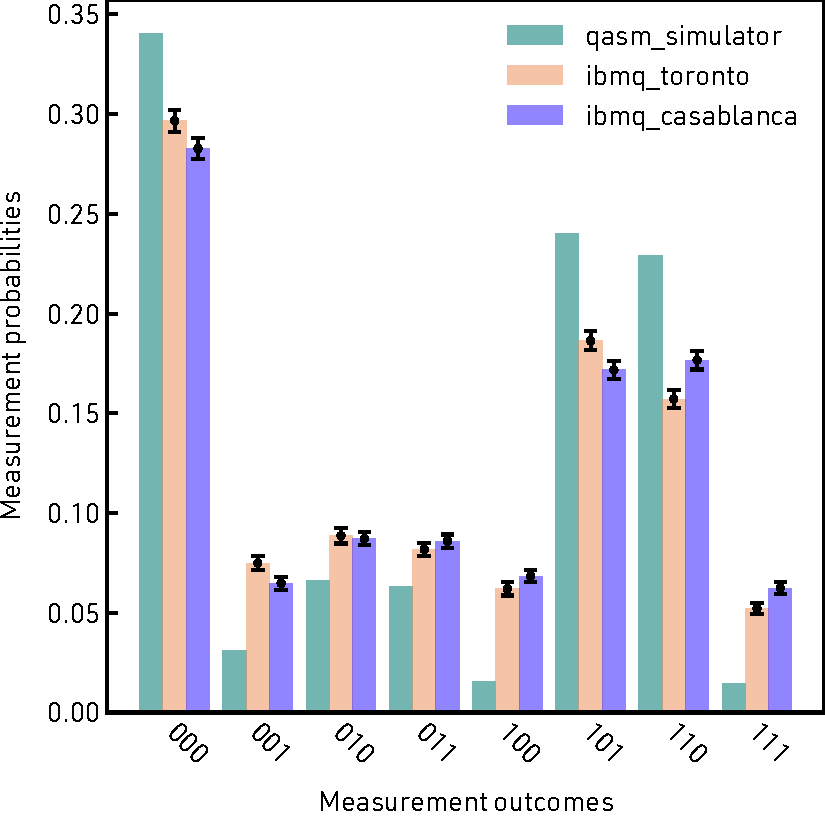
\includegraphics[width=0.86\textwidth]{shor_outcomes}
    \caption[Results of the complete quantum order-finding routine for ${N = 21}$ and ${x=4}$.]{Results of the complete quantum order-finding routine for ${N = 21}$ and ${x=4}$. On each processor, the circuit was executed ${8192 \times 100}$ times with measurement error mitigation. The error bars represent ${95\%}$ confidence intervals around the mean value of each histogram bin (see~\protect\refSectionOnly{error_bars} of technical~\protect\refAppendixOnly{appendix_B} details). The simulator probabilities show the ideal case.
    }
    \labelFigure{shor_outcomes}
\end{figure}

%p \begin{figure}[t!]
%     \centering
%     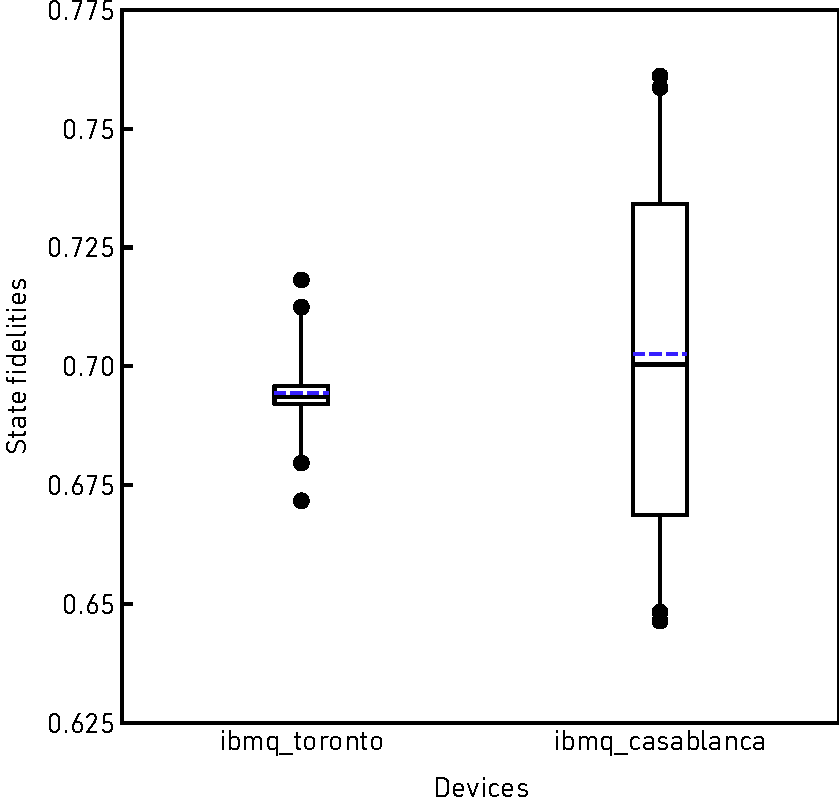
\includegraphics[width=0.90\textwidth]{shor_fidelities}
%     \caption[Boxplot of a sample ($\nu = 50$) of state fidelities from the respective two devices.]{Boxplot of a sample ($\nu = 50$) of state fidelities from the respective two devices showing the spread of the values around the sample mean and $95\%$ confidence intervals.}
%     \labelFigure{shor_box_plot}
% \end{figure}

\noindent
The theoretical ideal probability is close to $0.25$, as can be seen from the simulator results in~\refFigureOnly{shor_outcomes}. However, the amplification of the peaks $\ket{000}$, $\ket{101}$ and $\ket{110}$ is clearly visible from the processor outcomes. 

\bigskip
\noindent
We quantify the successful performance of the algorithm by comparing the experimental and ideal probability distributions \via the trace distance or Kolmogorov distance~\cite{Mike&Ike}, which measures the closeness of two discrete probability distributions $P$ and $Q$ and is defined by the equation $D(P,Q) \equiv \sum_{x \in \mathcal{X}}|P(x) - Q(x)|/2$, where ${\cal X}$ represents all possible outcomes. This measure shows an agreement between measured and ideal results -- the trace distance between the measured distribution and the ideal distribution is close to $0.1694$ and $0.1784$ for \textbf{ibmq\_toronto} and \textbf{ibmq\_casablanca}, respectively. On the other hand, the trace distance between the ideal distribution and a candidate random uniform distribution is $0.4347$. Furthermore, we evaluate the performance of the algorithm by characterizing the measured output state in the control register, this is achieved \via state tomography yielding the density matrix of the measured state. The measured state and ideal state on the output register are quantitatively compared using the fidelity for two quantum states $\varrho$ and $\var$, and is defined to be $F(\varrho, \varsigma) \equiv \Tr(\sqrt{\sqrt{\varrho}\varsigma\sqrt{\varrho}}^2)$~\cite{Mike&Ike}. We measured a fidelity of $F(\varrho_\text{id}, \varrho_{27Q})=0.6948 \pm 00650$ and $F(\varrho_\text{id}, \varrho_{7Q}) = 0.70 \pm 0.0275$ on the $27$ qubit and $7$ qubit quantum processors respectively. In~\refFigureOnly{shor_density_mats} we show the estimated density matrices in the computational basis for each respective device.

\clearpage

\begin{figure*}[t!]
    \centering
	\subfloat[\labelFigure{shor_mat2d_ideal_real}]
	{
		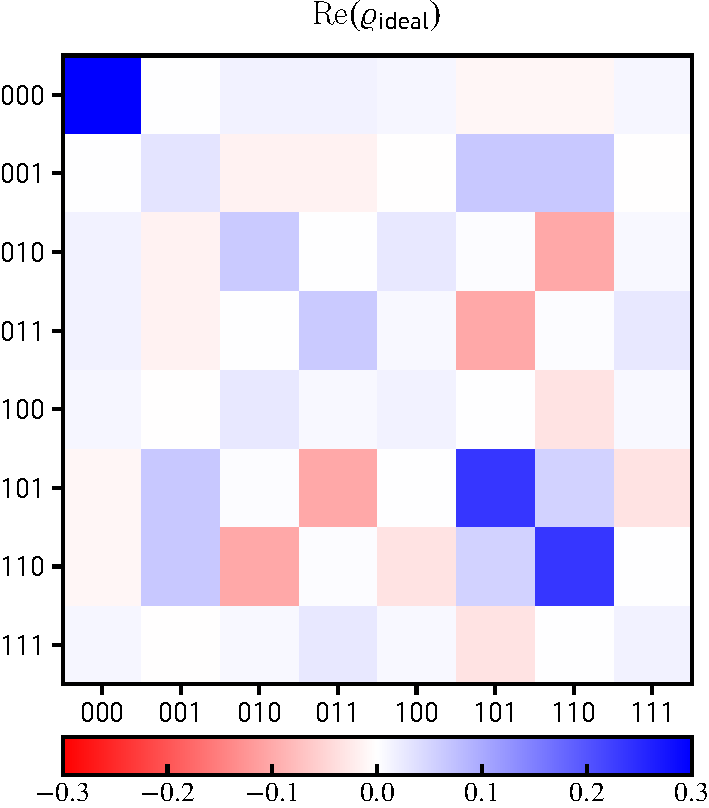
\includegraphics[width=0.5\textwidth]{shor_mat2d_ideal_real}
	}
	\subfloat[\labelFigure{shor_mat2d_ideal_imaginary}]
	{
		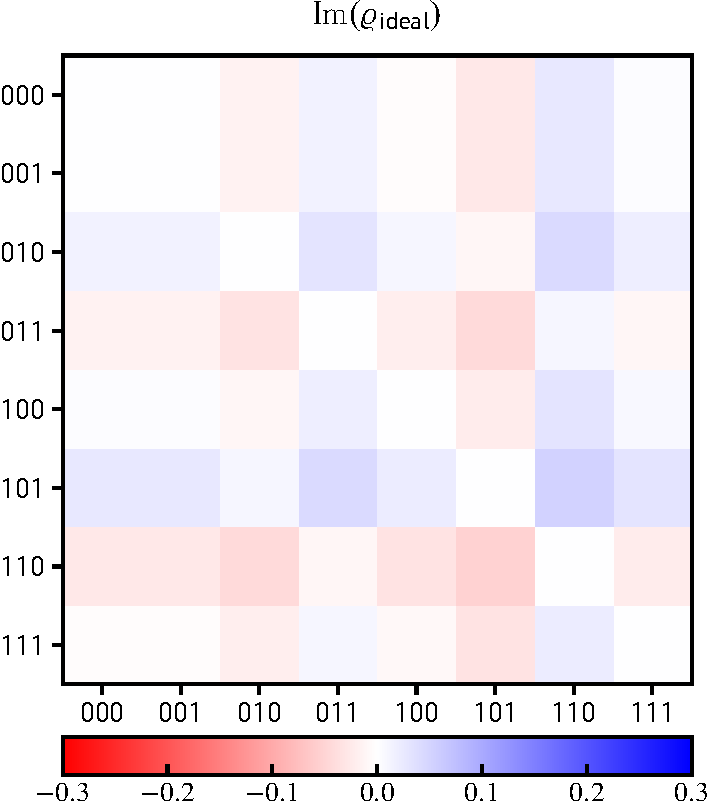
\includegraphics[width=0.5\textwidth]{shor_mat2d_ideal_imaginary}
	} \\
	\subfloat[\labelFigure{shor_mat2d_toronto_real}]
	{
		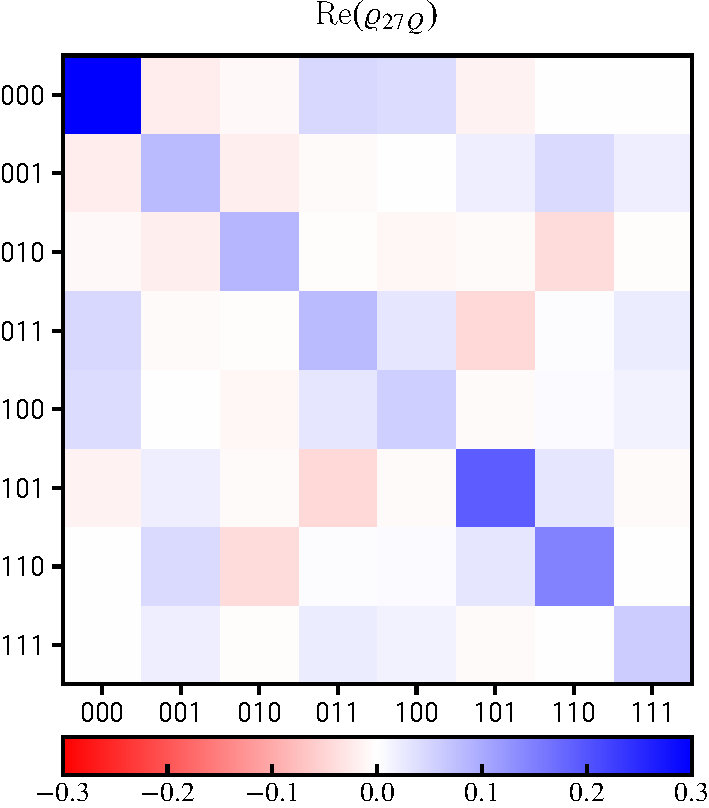
\includegraphics[width=0.5\textwidth]{shor_mat2d_toronto_real}
	}
	\subfloat[\labelFigure{shor_mat2d_toronto_imaginary}]
	{
		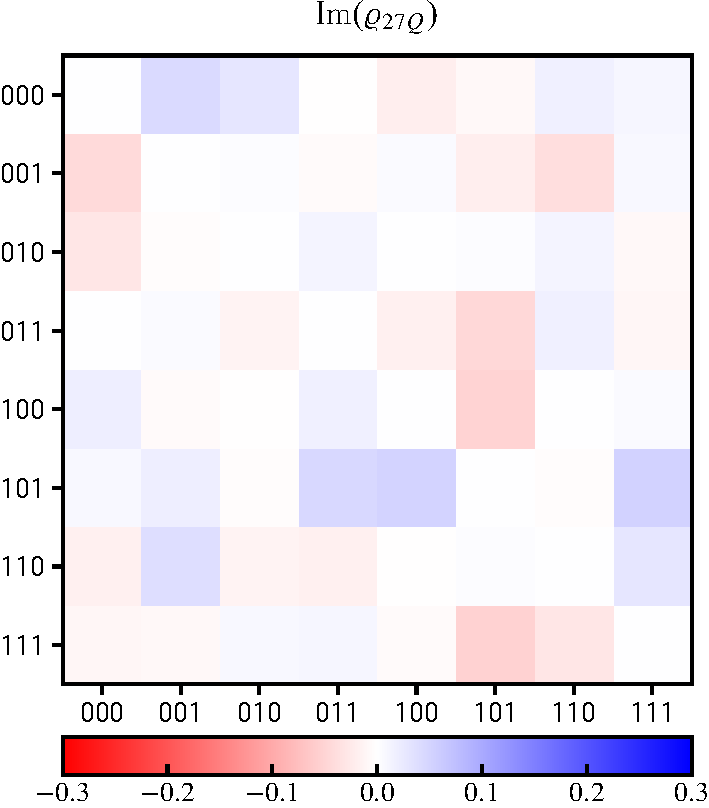
\includegraphics[width=0.5\textwidth]{shor_mat2d_toronto_imaginary}
	}
\end{figure*}

\clearpage

\begin{figure*}[t!]
	\addtocounter{subfigure}{4}
	\subfloat[\labelFigure{shor_mat2d_casablanca_real}]
	{
		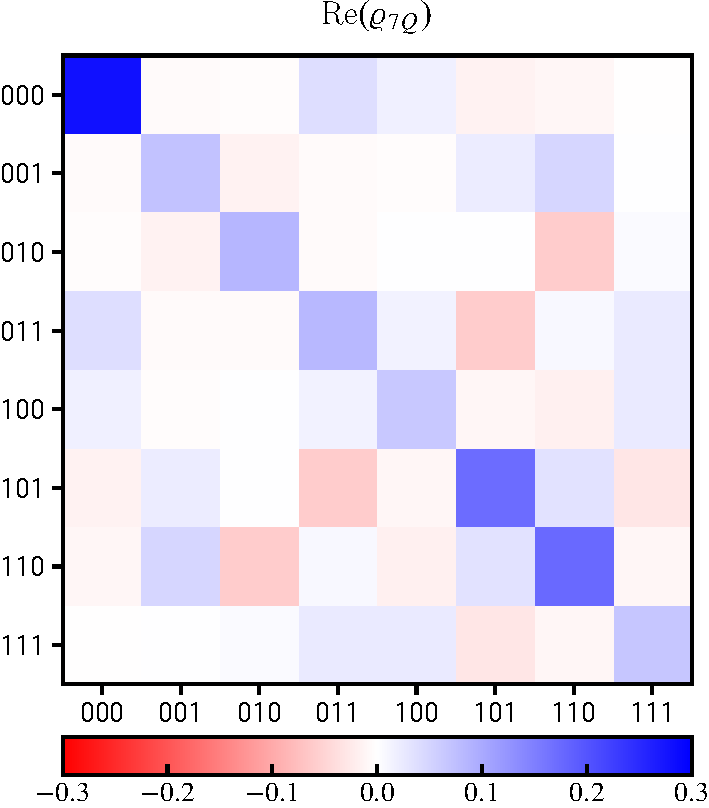
\includegraphics[width=0.5\textwidth]{shor_mat2d_casablanca_real}
	}
	\subfloat[\labelFigure{shor_mat2d_casablanca_imaginary}]
	{
		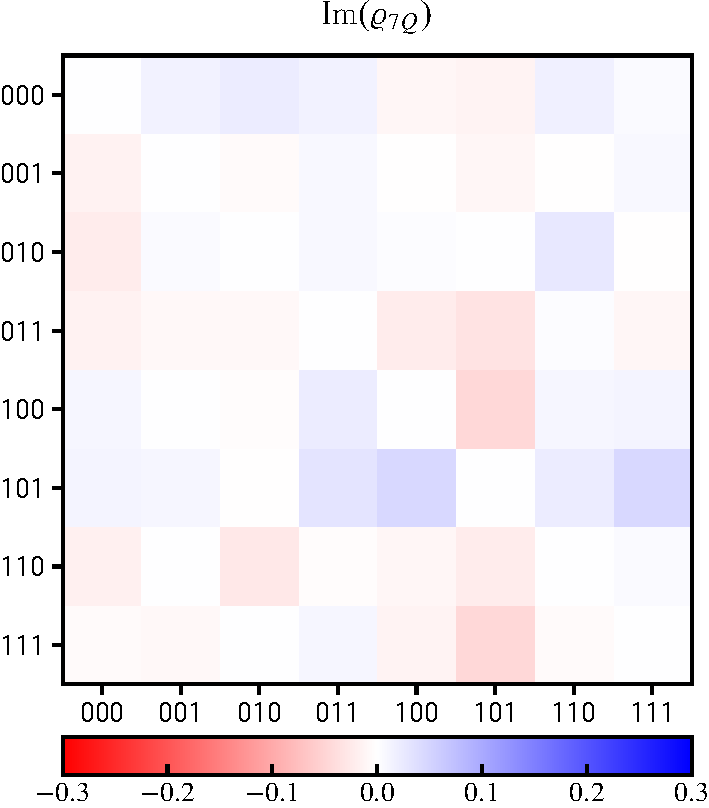
\includegraphics[width=0.5\textwidth]{shor_mat2d_casablanca_imaginary}
	}
    \caption[Ideal and measured density matrices after the inverse \acs{QFT}, estimated \via a maximum-likelihood reconstruction from measurement results in the Pauli-basis.]{Ideal and measured density matrices after the inverse \acs{QFT}, estimated \via a maximum-likelihood reconstruction from measurement results in the Pauli-basis. A matrix plot of the \textbf{(a)} real and \textbf{(b)} imaginary part of the ideal state $\op{\Psi}$. These plots are compared with the measured states $\rho_{27Q}$ and $\rho_{7Q}$ with the corresponding matrix plots of their real parts in panels \textbf{(c)} and \textbf{(e)}, and imaginary parts in panels \textbf{(d)} and \textbf{(f)}, respectively. We observe there is a resemblance between the ideal state and the measured states, but noise in both real and imaginary parts is notable. Note that in all figures the color bar has been rescaled to a range between $-0.3$ and $0.3$ for visual clarity.}
    \labelFigure{shor_density_mats}
\end{figure*}

\subsection{Factoring $N=21$}
\labelSection{C3_factoring_n_21}

The measured probability distributions in~\refFigureOnly{shor_outcomes} are peaked in probability for the outcomes $000~(\varphi_s=0)$, $101~(\varphi_s=5)$ and $110~(\varphi_s=6)$, with ideal probabilities of $0.35$, $0.25$ and $0.25$, respectively. Here we are using the integer representation of the binary outcomes. The outcome $000$ corresponds to a failure of the algorithm~\cite{Lopez_2012}. For the outcome $101$, computing the continued fraction expansion of $\varphi=\varphi_s/2^n=5/2^3=5/8$ gives the convergents $\{0, 1, 1/2, 2/3, 5/8\}$ (see~\refSectionOnly{continued_fractions} of  technical~\refAppendixOnly{appendix_B} for details), so that the third convergent $2/3$ in the expansion can be identified as $s/r$ and correctly gives $r=3$ as the order when tested with the relation $x^r \text{ mod } N=1$, while the other convergents do not give an $r$ that passes the test. On the other hand, the continued fraction expansion of $\varphi=6/8$ gives $\{0, 1, 3/4\}$ and incorrectly gives $r=4$ as the order (see~\refSectionOnly{continued_fractions} of technical~\refAppendixOnly{appendix_B} for details). This failure can be avoided in principle by adding further qubits to the control register so that the peak in the probability distribution becomes narrower and more well defined~\cite{Lopez_2012}. Another option is to simply apply continued fractions to all peaked outcomes and test if the value of $r$ found satisfies the order relation for $x$ and $N$. It is interesting to note that from the results of Ref.~\cite{Lopez_2012}, successfully finding the order $r=3$ was not possible to achieve, as with only two bits of accuracy in the experiment the continued fractions would always fail due to the peaked outcomes of $10~(2)$ and $11~(3)$ giving the convergents of $\{0,1/2\}$ and $\{0,1,3/4\}$, respectively. In our case, we successfully find $r=3$, from which we obtain $\gcd(x^{r/2}\pm1,N)=\gcd(8\pm1,21)=3$ and 7. Thus, with our demonstration, extending the number of outcome bits to three has allowed us to fully perform the quantum factoring of $N=21$.


%%%%%%%%%%%%%%%%%%%%%%%%%%%
%%%%%%%%%%%%%%%%%%%%%%%%%%%

\clearpage
\subsection{Verification of entanglement}
\labelSection{C3_verification_of_entanglement}

The presence of entanglement between the control and work registers is known to be a requirement for the algorithm to gain any advantageous speedup over its classical counterpart in general~\cite{Vidal_2003a, Braunstein_1999, Jozsa_2003}. For detecting genuine multipartite entanglement around the vicinity of an ideal state $\ket{\psi}$, one can construct a projector-based witness such as the one below:

\begin{align}
    \hat{\mathcal{W}}_{\psi} = \alpha \mathds{1} - \op{\psi}{\psi},
\end{align}

\noindent
where $\alpha$ is the square of the maximum overlap between $\ket{\psi}$ and all biseparable states. In other words, $\Tr(\hat{\mathcal{W}}_{\psi}\varrho) \geq 0$ for biseparable states and $\Tr(\hat{\mathcal{W}}_{\psi}\varrho) < 0$ for states with genuine multipartite entanglement in the vicinity of $\ket{\psi}$~\cite{Bourennane_2004}. For the ideal state after modular exponentiation (but before the inverse \acs{QFT}) in both the control and work registers, $\alpha=0.75$ was found using the method described in the appendix of Ref.~\cite{Bourennane_2004}. This was implemented using the software package QUBIT4MATLAB~\cite{Toth_2008}. Therefore ideally the state in both registers after modular exponentiation has genuine multipartite entanglement.

\bigskip
\noindent
In order to check whether the output state from the IBM processors is close to the ideal state and has genuine multipartite entanglement, full state tomography would normally be needed to characterize the state $\varrho_\text{exp}$ in both the control and work registers. This would require $3^5$ measurements, making it impractical to gather a sufficiently large data set within a meaningful time frame. However, we need not measure the full density matrix, the quantity $\Tr(\op{\Psi}{\Psi}\varrho_\text{exp})$ suffices. To measure this, we can decompose $\varrho=\op{\Psi}{\Psi}$ into $293$ Pauli terms as

\begin{align}
    \op{\Psi}{\Psi} = \displaystyle\sum_{ijklm} p_{ijklm} \sigma_i^{(1)}\sigma_j^{(2)}\sigma_k^{(3)}\sigma_l^{(4)}\sigma_m^{(5)},
\end{align}

\noindent
where $\sigma_{i} = \{I, X, Y, Z\}$ are the usual Pauli matrices plus the identity. 

\bigskip

\noindent
However, the number of measurements needed to obtain all 293 expectation values can be reduced. This is because the measured probabilities from a measurement of a single Pauli expectation value, \ie $\expval{ZZZZZ}$, can be summed in various combinations to derive other Pauli expectations values, \ie $\expval{ZIZZZ}, \expval{IZZZZ}$, etc. The values derived are nothing but the marginalization of the measured probabilities over the outcome space of some set of qubits (see~\refSectionOnly{pauli_measurements} of technical~\refAppendixOnly{appendix_B} for details). We can do the same for each term in the set of terms from the Pauli decomposition of $\varrho$, calling it $\mathcal{S}_d$, forming a set of other Pauli terms that can be derived from the same counts. Taking the union of these sets to be $\mathcal{S}_u$, the complement $\mathcal{S}_d\setminus\mathcal{S}_u$ gives the $79$ terms we only need to measure (see~\refSectionOnly{pauli_measurements} of technical~\refAppendixOnly{appendix_B} for details). We measure the 79 Pauli expectation values of the terms above with respect to the state in both registers after modular exponentiation and from this we compute/derive the $293$ terms in $\mathcal{S}_d$ and therefore $\Tr(\op{\Psi}{\Psi}\varrho_\text{exp})$; the measurement outcomes for evaluating some of the Pauli operator expectation values are shown in~\refFigureOnly{klocals}. 

\clearpage
\noindent
The measured probabilities for each term result in an expectation value of $\Tr(\op{\Psi}{\Psi}\varrho_{7Q}) = 0.677 \pm 0.00365$ and $\Tr(\op{\Psi}{\Psi}\varrho_{27Q}) = 0.626 \pm 0.00304$, which leads to

\begin{align}
  \Tr(\hat{\mathcal{W}}_{\Psi}\varrho_{7Q})  &= 0.0729 \pm 0.00365,\nonumber \\
  \Tr(\hat{\mathcal{W}}_{\Psi}\varrho_{27Q}) &= 0.124 \pm 0.00304.
\end{align}

\noindent
The results obviously fail to detect genuine multipartite entanglement, however, this does not mean entanglement is entirely absent. Consider the square of the maximum overlap between the ideal state $\ket{\Psi}$ and all pure states $\ket{\theta}$ that are unentangled product states with respect to some bipartite partition (bipartition) $\mathcal{B}$ of the qubits,

\begin{align}\labelEquation{maximal_overlap}
    \underset{\theta \in \mathcal{B}}{\max}{\abs{\ip{\theta}{\Psi}}^2} = \beta_{\Psi}.
\end{align}

\noindent
Thus, any other state $\ket{\xi}$ for which 

\begin{align}
    \abs{\ip{\xi}{\Psi}}^2 > \beta_{\Psi},
\end{align}

\noindent
cannot be a product state with respect to the bipartition $\mathcal{B}$, implying that there is non-separability, or entanglement, across this bipartition. The above result extends to mixed states $\varrho_\xi$ due to the convex sum nature of mixed quantum states~\cite{Toth_2008}. We compute \refEquationOnly{maximal_overlap} for all possible bipartitions of our ideal state $\ket{\Psi}$ (see~\refSectionOnly{maximum_overlap_wrt_bipartitions} of technical~\refAppendixOnly{appendix_B} for details). 

\bigskip
\noindent
For the experimental state $\varrho_{7Q}$ we find, with the exception of the bipartition $\mathcal{B}=(c_0c_1c_2q_1)(q_0)$, that it is non-separable with respect to all other bipartitions, \ie the square of the overlap between $\varrho_{7Q}$ and $\ket{\Psi}$ ($\sim 0.677$) is greater than the maximal square overlap between $\ket{\Psi}$ and all product states in each of these bipartitions. Similarly for $\varrho_{27Q}$, with the exception of bipartitions $\mathcal{B}=(c_0c_1c_2q_1)(q_0)$ and $\mathcal{B}=(c_0c_1c_2q_0)(q_1)$, the state is non-separable with respect to all other bipartitions. Most notably, both $\varrho_{7Q}$ and $\varrho_{27Q}$ are non-separable with respect to the bipartition ${\cal B}=(c_0c_1c_2)(q_0q_1)$, which is a bipartition between the control and work registers. 


% Another signature of non-separability between bipartitions of a pure state $\ket{\psi}$ is given by the entropy of entanglement~\cite{Bennett_1996},

% \begin{align}
% 	\mathcal{S}(\varrho_A) = -\tr(\varrho_a \log \varrho_A),
% \end{align}

% \noindent
% where $\varrho_A = \tr_B(\op{\psi})$ is the reduced density matrix of subsystem A of $\ket{\psi}$. If $\ket{\psi}$ is separable with respect to this bipartition, \ie $\ket{\psi} = \ket{\phi_A}\ket{\phi_B}$, then $\varrho_A = \op{\phi_A}$ is pure state for which the entropy of entanglement is $\mathcal{S}(\op{\phi_A}) = 0$; thus a non-zero entropy of entanglement indicative of non-separability between the two consideration bipartitions of $\ket{\psi}$.  We measure entropy of entanglement for our density matrix estimates (after the inverse \acs{QFT}) of the control register subsystem on each device, and find $\mathcal{S}(\varrho_{27Q}) = 1.659\pm0.0154$ $\mathcal{S}(\varrho_{7Q}) = 1.765\pm0.0387$,  respectively for the two devices.

% \bigskip
% \noindent
% This implies that non-separability or entanglement is present between the registers before (and after) the \acs{QFT}, as required for the algorithm's speedup in general~\cite{Vidal_2003a, Braunstein_1999, Jozsa_2003}. Furthermore, the maximum (not necessarily global but a good proxy of it) expectation value of the operator $\op{\Psi}{\Psi}$ for product states, is found \via a greedy search algorithm~\cite{Toth_2008} to be around $0.30$, further asserting that indeed the qubits are entangled with each other in some way.

\begin{figure*}[h!]
	\subfloat[\labelFigure{casablanca_klocals}]
	{
        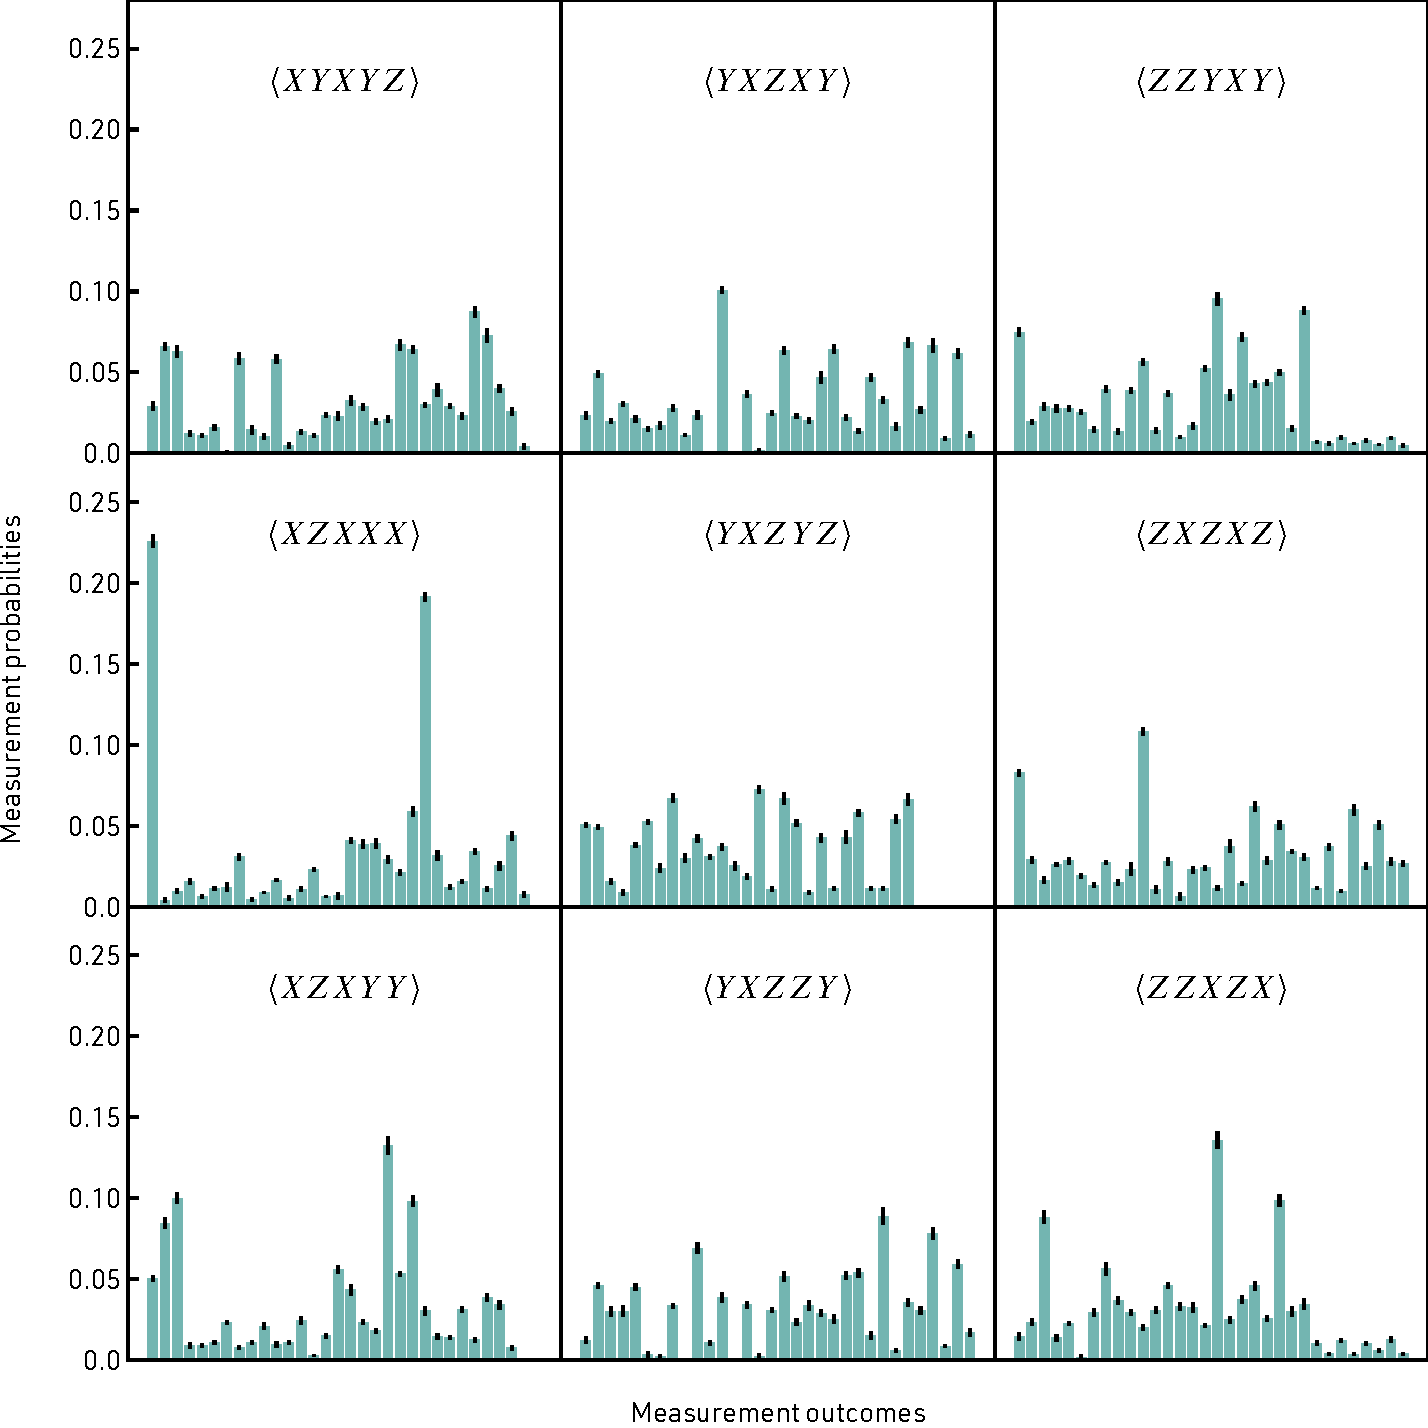
\includegraphics[width=\textwidth]{klocals_casablanca}
	}
\end{figure*}

\clearpage

\begin{figure*}[t!]
	\addtocounter{subfigure}{1}
	\subfloat[\labelFigure{toronto_klocals}]
	{
        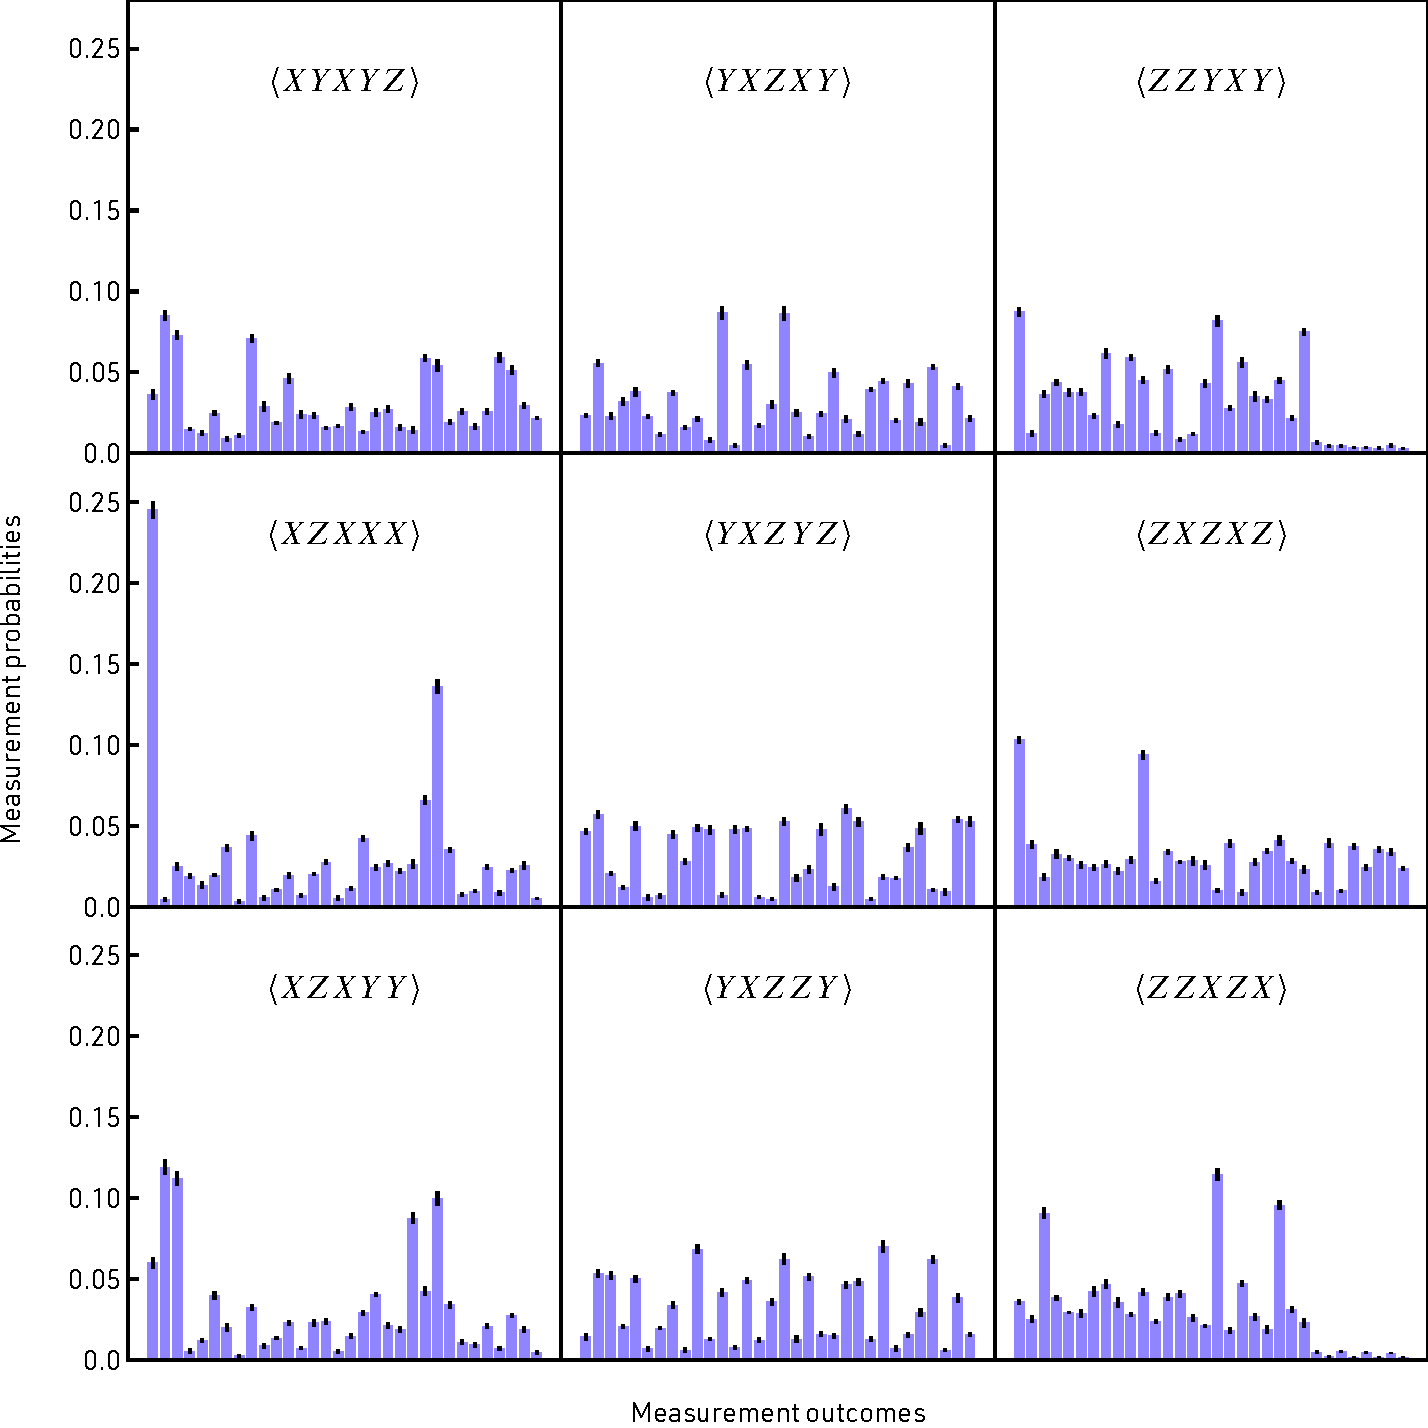
\includegraphics[width=\textwidth]{klocals_toronto}
	}
    \caption[A subset of 9 of the 79 measurement settings.]{A subset of 9 of the 79 measurement settings required for each term in: \textbf{(a)} $\Tr(\op{\Psi}{\Psi}\varrho_{7Q})$ and \textbf{(b)} $\Tr(\op{\Psi}{\Psi}\varrho_{27Q})$. The $x$-axis from left to right shows the labels from $p_{00000}$ to $p_{11111}$.}
    \labelFigure{klocals}
\end{figure*}

\clearpage

\section{Concluding remarks}
\labelSection{C3_concluding_remarks}
In summary, we have implemented a compiled version of Shor's algorithm on IBM's quantum processors for the prime factorization of $21$. By using relative phase shift Toffoli gates, we were able to reduce the resource demands that would have been required in the standard compiled and non-iterative construction of Shor's algorithm (with regular Toffoli gates), and still preserve its functional correctness. The use of relative phase shift Toffoli gates has also allowed us to extend the implementation in Ref.~\cite{Lopez_2012} to an increased resolution. Moreover, while the latter implementation used only 1 recycled qubit for the control register, in contrast to our 3 qubits, it falls one iteration short of achieving full factoring for the reasons already mentioned. It is not clear what additional resource overheads (single and two-qubit gates) would be needed in implementing another iteration in their scheme and it is likely that these overheads are what prevented the full factoring of 21 in the photonic setup used. Furthermore, we note that in principle there is no real advantage in using 3 qubits for the control register as we have done here instead of 1 qubit recycled, as in Ref.~\cite{Lopez_2012}. However, in practice it is not possible at present to recycle qubits on the IBM processors and so we used 3 qubits instead. In future, once this capability is added, a further reduction in resources will be possible for our implementation, potentially improving the quality of the results even more. 

\bigskip
\noindent
We have verified, \via state tomography, the output state in the control register for the algorithm, achieving a fidelity of around $0.70$. For the verification of entanglement generated during the algorithm's operation, the resource demands of state tomography were circumvented by measuring a much reduced number of Pauli measurements to directly estimate the fidelity of the state. However, this method is quite specialized and cannot be easily generalized to larger systems. In scaling up Shor's algorithm to higher integers beyond 21 using larger quantum systems, other methods of quantum tomography / direct fidelity estimation can be used to characterize the performance. These include compressed sensing~\cite{Gross_2010} and classical shadows~\cite{Huang_2020}, which give theoretical guarantees, and improved scaling in the number of Pauli measurements and classical post-processing than standard methods. In the case where one is only interested in a direct estimate of fidelity, the method due to Flammia and Liu~\cite{Flammia_2011} provides a fidelity estimate using a constant number of Pauli expectation values. 


\bigskip
\noindent
For states that belong to a class of states with certain symmetries, such as stabilizer states, only a few measurements are required for measuring the fidelity and detecting multipartite entanglement~\cite{Toth_2005}. However, not all entangled states are neatly housed within these well-studied classes. Ref.~\cite{Baccari_2017} introduces a device-independent method for multipartite entanglement detection which scales polynomially with the system size by relaxing some constraints. Another scheme constructs witnesses that require a constant number of measurements of the system size at the cost of robustness against white noise. This provides a fast and simple procedure for entanglement detection~\cite{Knips_2016}. Many fundamental questions on the subjects of quantum tomography and multipartite entanglement still remain to be answered~\cite{Banaszek_2013} and advances will help in efficiently quantifying the performance of algorithms in larger quantum processors.


\bigskip
\noindent
Our demonstration involves a two-fold reduction of the resource count from the full circuit in~\refFigureOnly{compiled_circ} \via the replacement of regular Toffoli gates with relative phase variants, which is an approach that is in the spirit of the NISQ era; tailoring quantum circuits to circumvent the shortcomings of noisy quantum processors. 

\clearpage
\noindent
 In addition, the resource count of the full \acs{QFT} in our circuit may be reduced through the use of the approximate \acs{QFT}~\cite{Barenco_1996}, while possibly still maintaining a clear resolution of the peaks in the output probability distribution~\cite{Coppersmith_2002}. A possible avenue of future research derived from what we have reported here is the investigation and identification of scenarios where one can replace Toffoli gates with relative phase Toffoli gates while preserving the functional correctness, in a wide range of algorithms including Shor's algorithm, as seen here. In the present case, whether such an approach is special to the case of $N=21$ or extendable to other $N$ is not known. Ref.~\cite{Maslov_2016} has performed some work in this regard, however a proper analysis and systematic composition of relative phase Toffoli gates for such purposes is still an open problem. In future, a similar approach may make possible the factorization of larger numbers with adequate accuracy in resolution of the algorithm's outcomes and their characterization.

%%%%%%%%%%%%%%%%%%%%%%%%%%%
%%%%%%%%%%%%%%%%%%%%%%%%%%%
%%%%%%%%%%%%%%%%%%%%%%%%%%%
